\documentclass{pginz}

%%%%%%%%% Miejsce na dodatkowe pakiety %%%%%%%%%%%%%
\usepackage{fontspec} % Pakiet do obsługi czcionek systemowych
\setmainfont{Arial} % Ustawienie Arial jako głównej czcionki
\usepackage{subcaption}
\usepackage{algorithm}
\usepackage{algpseudocode}
\usepackage[numbers]{natbib}
\usepackage{multirow}
\usepackage{booktabs}
\usepackage{float}
\begin{document}

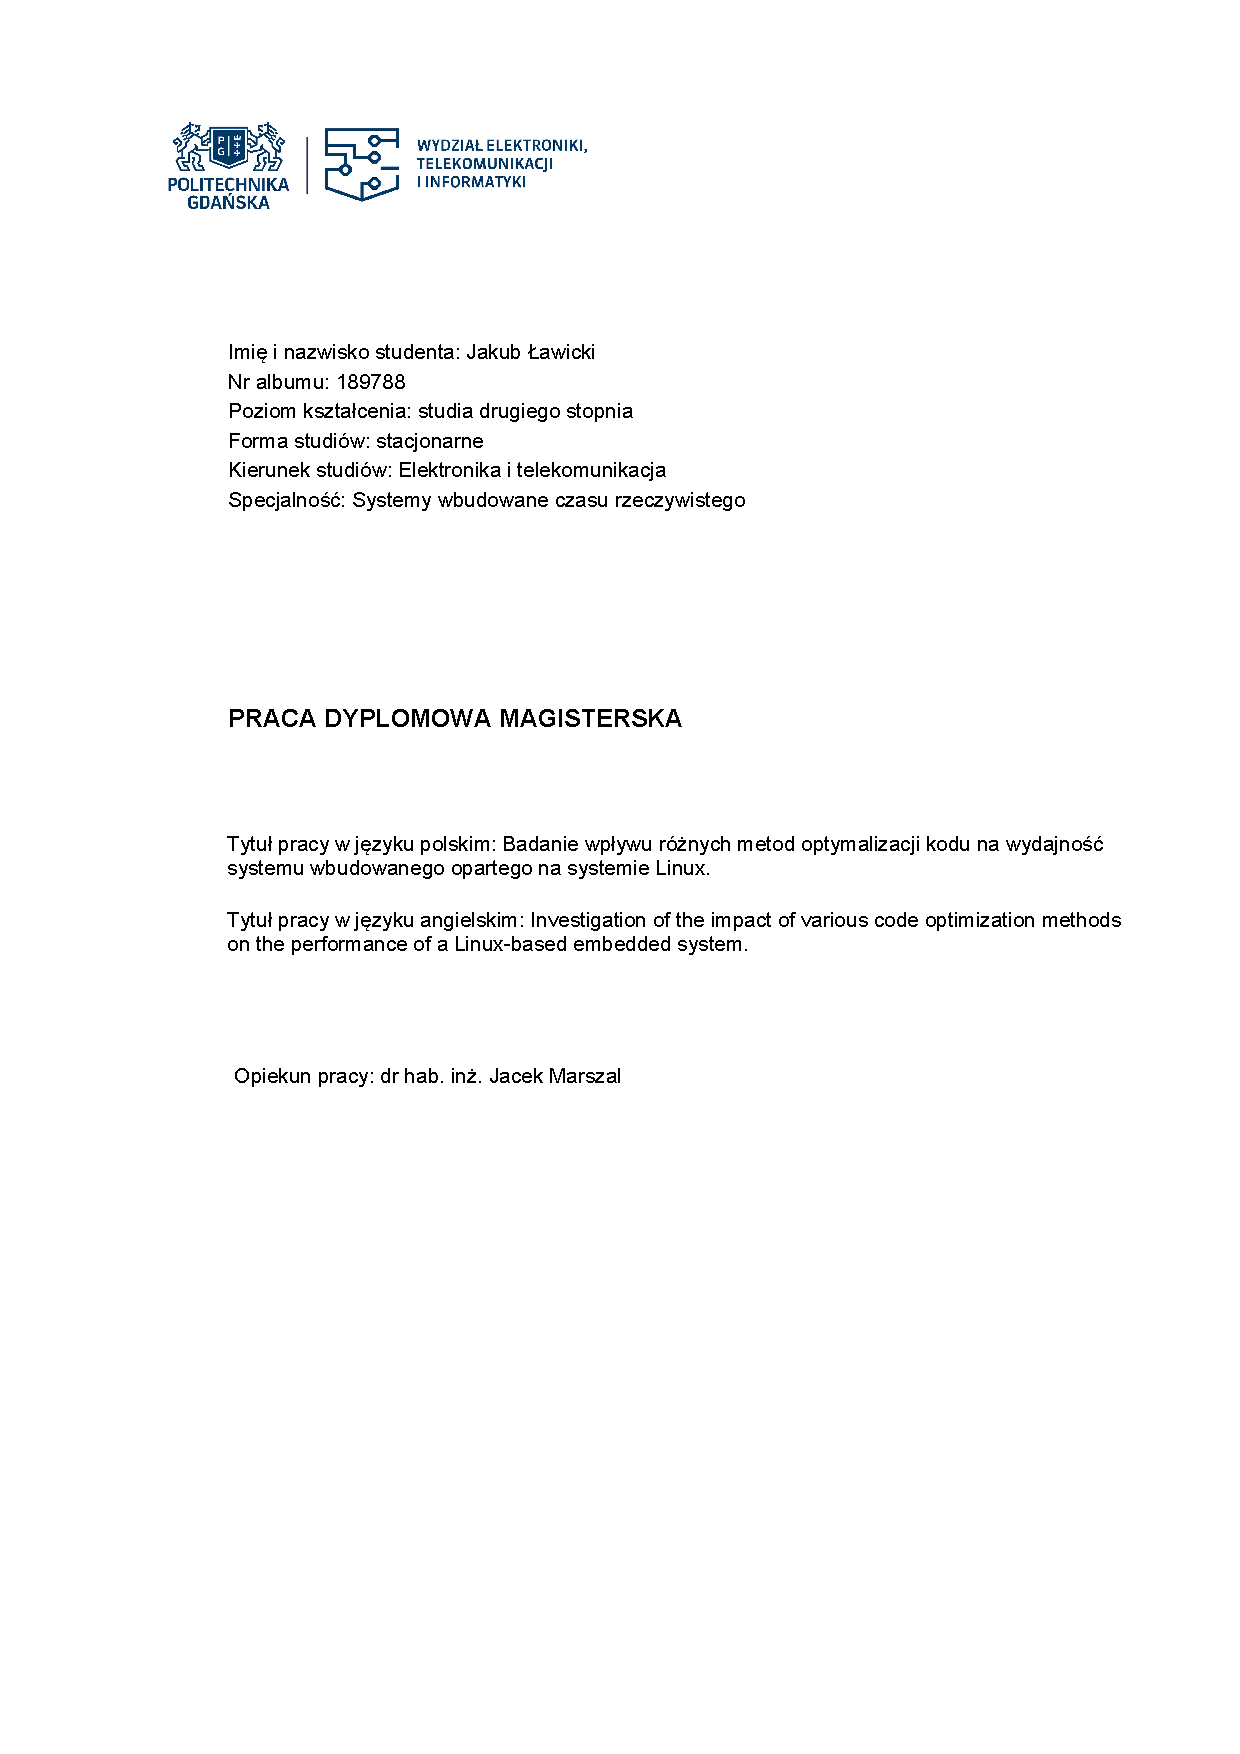
\includepdf[]{StronaTytulowa.pdf}
%\includepdf[page={1}]{Oswiadczenie.pdf}
\setcounter{page}{2}

\chapter*{Streszczenie}
Kompilator jest niezbędnym narzędziem przy tworzeniu programów komputerowych,
które efektywnie wykorzystują zasoby sprzętowe systemu. Bywa on jednak
traktowany jedynie jako tłumacz kodu, z~pominięciem jego możliwości
optymalizacyjnych, choć sposób tłumaczenia kodu źródłowego na instrukcje
maszynowe wpływa bezpośrednio na wydajność programu.

Zagadnienie to ma szczególne znaczenie w~systemach
wbudowanych, w~których poprawa wydajności oznacza często niższy
koszt i~mniejszy pobór energii. W~prezentowanej pracy zaprojektowano system
wbudowany oparty na platformie Raspberry Pi 4B z~systemem Linux, przeznaczony do
badania możliwości optymalizacyjnych kompilatorów GCC i~Clang. Jako algorytm
testowy wybrano szybką transformatę Fouriera, dla której zaimplementowano
w~języku C jedenaście wariantów, zarówno sekwencyjnych jaki~wielowątkowych. 

W~pracy zawarto również opis systemów operacyjnych w~zastosowaniach wbudowanych, podstaw
transformaty Fouriera oraz budowy kompilatora i~stosowanych przez niego
optymalizacji. Badania objęły jedenaście zestawów flag kompilacji i~trzy
rozmiary danych wejściowych, a~oprócz czasu wykonania analizowano liczniki
sprzętowe, rozmiar kodu wynikowego oraz dokładność obliczeń.

Największy zysk
przyniosło odejście od domyślnego poziomu \texttt{-O0}, które skróciło czas
wykonania od 2,18 do 5,11 raza, podczas gdy dalszy dobór flag dawał zwykle
około 12\%. Dla dużych zbiorów danych o~czasie wykonania decydował przede
wszystkim wzorzec dostępu do pamięci, dlatego wybór schematu obliczeń okazał
się równie istotny jak poziom optymalizacji. Ręczna wektoryzacja z~użyciem
instrukcji NEON oraz zrównoleglenie obliczeń przynosiły wyraźne korzyści tylko
w~określonych zakresach rozmiaru danych. Kompilator nie skorygował przy tym
błędów numerycznych wynikających z~konstrukcji algorytmu. Uzyskane wyniki
wskazują, że optymalizację programu należy zaczynać od doboru algorytmu
i~organizacji danych, a~ustawienia kompilacji traktować jako ich uzupełnienie.

\bigskip

\noindent\textbf{Słowa kluczowe:} optymalizacja kompilacji, kompilatory GCC i~Clang, szybka transformata Fouriera, systemy wbudowane, system operacyjny Linux

\bigskip

\noindent\textbf{Dziedzina nauki i techniki zgodna z OECD} Nauki inżynieryjne i techniczne, Elektrotechnika, elektronika i inżynieria informatyczna,

\chapter*{Abstract}
The compiler is an essential tool in the development of computer programs that
make efficient use of the system's hardware resources. It is often treated,
however, as a mere code translator, with its optimization capabilities left
aside, even though the way source code is translated into machine instructions
directly affects program performance.

This issue is of particular importance in embedded systems, where improved
performance often means lower cost and reduced power consumption. This thesis
presents an embedded system based on the Raspberry Pi 4B platform running Linux,
designed to study the optimization capabilities of the GCC and Clang compilers.
The fast Fourier transform was chosen as the test algorithm, for which eleven
variants were implemented in C, both sequential and multithreaded.

The thesis also covers operating systems in embedded applications, the
fundamentals of the Fourier transform, and the structure of a compiler together
with the optimizations it applies. The study covered eleven sets of compilation
flags and three input data sizes; in addition to execution time, hardware
counters, output code size, and computational accuracy were analysed.

The largest gain came from moving away from the default \texttt{-O0} level,
which reduced execution time by a factor of 2.18 to 5.11, whereas further flag
selection typically yielded around 12\%. For large data sets, execution time was
determined mainly by the memory access pattern, which made the choice of
computational scheme as important as the optimization level. Manual
vectorization using NEON instructions and parallelization of the computation
brought clear benefits only within specific ranges of data size. The compiler
did not correct numerical errors resulting from the construction of the
algorithm. The results indicate that program optimization should begin with the
choice of algorithm and data organization, with compilation settings treated as
a complement to them.

\bigskip

\noindent\textbf{Keywords:} compilation optimization, GCC and Clang compilers,
fast Fourier transform, embedded systems, Linux operating system

\bigskip

\noindent\textbf{OECD consistent field of science and technology classification:} Engineering and technology, Electrical engineering, Electronic engineering, Information engineering, 


\tableofcontents
\addcontentsline{toc}{chapter}{Spis treści}

\chapter*{Lista symboli}

\begin{itemize}[noitemsep,topsep=0pt,parsep=0pt,partopsep=0pt,labelwidth=2cm,leftmargin=2.3cm,align=left,itemindent=0pt]
\item[\(N\)] - liczba próbek transformaty
\item[\(n\)] - indeks próbki w dziedzinie czasu
\item[\(k\)] - indeks prążka widma
\item[\(x(n)\)] - \textit{n}-ta próbka sygnału dyskretnego
\item[\(X(k)\)] - \textit{k}-ty prążek widma dyskretnego
\item[\(W_N\)] - czynnik obrotu transformaty o długości \(N\)
\item[\(p,\, q\)] - pozycje dwóch elementów przetwarzanych w operacji motylkowej
\item[\(s\)] - numer etapu algorytmu FFT
\item[\(t_{1/2}\)] - mediana czasu wykonania transformaty
\item[\(Q_1,\, Q_3\)] - pierwszy i trzeci kwartyl czasu wykonania
\item[\(t_{\mathrm{CPU}}\)] - sumaryczny czas procesora
\item[\(t_{\mathrm{wall}}\)] - czas ściany, czyli rzeczywisty czas trwania obliczeń
\item[\(R\)] - stosunek czasu procesora do czasu ściany
\item[\(I\)] - liczba wykonanych instrukcji
\item[\(C\)] - liczba cykli procesora
\item[\(m\)] - współczynnik chybień danego poziomu pamięci podręcznej
\item[\(r,\, a\)] - liczba chybień i liczba odwołań do danego poziomu pamięci podręcznej
\item[\(v\)] - udział instrukcji wektorowych w kodzie wynikowym
\item[\(n_{\mathrm{SIMD}},\, n_{\mathrm{skal}}\)] - liczba instrukcji wektorowych i skalarnych
\item[\(X_k,\, X_k^{\mathrm{ref}}\)] - \textit{k}-ty prążek widma badanego wariantu i widma referencyjnego
\end{itemize}

\chapter*{Lista skrótów}

\begin{itemize}[noitemsep,topsep=0pt,parsep=0pt,partopsep=0pt,labelwidth=2cm,leftmargin=2.3cm,align=left,itemindent=0pt]
\item[AoS] - układ złożony danych (ang. \textit{Array of Structures})
\item[DFT] - dyskretna transformacja Fouriera (ang. \textit{Discrete Fourier Transform})
\item[DIF] - decymacja w dziedzinie częstotliwości (ang. \textit{Decimation in Frequency})
\item[DIT] - decymacja w dziedzinie czasu (ang. \textit{Decimation in Time})
\item[FFT] - szybka transformacja Fouriera (ang. \textit{Fast Fourier Transform})
\item[FFTW] - biblioteka szybkiej transformacji Fouriera (ang. \textit{Fastest Fourier Transform in the West})
\item[GCC] - zestaw kompilatorów projektu GNU (ang. \textit{GNU Compiler Collection})
\item[IPC] - liczba instrukcji wykonanych w jednym cyklu (ang. \textit{Instructions Per Cycle})
\item[IQR] - rozstęp międzykwartylowy (ang. \textit{Interquartile Range})
\item[LLVM] - infrastruktura budowy kompilatorów (ang. \textit{Low Level Virtual Machine})
\item[LTO] - optymalizacja na etapie konsolidacji (ang. \textit{Link Time Optimization})
\item[MMU] - jednostka zarządzania pamięcią (ang. \textit{Memory Management Unit})
\item[NEON] - jednostka wektorowa architektury ARM (ang. \textit{Advanced SIMD})
\item[POSIX] - przenośny interfejs systemów operacyjnych (ang. \textit{Portable Operating System Interface})
\item[RMSE] - pierwiastek błędu średniokwadratowego (ang. \textit{Root Mean Square Error})
\item[RTOS] - system operacyjny czasu rzeczywistego (ang. \textit{Real-Time Operating System})
\item[SIMD] - pojedynczy strumień instrukcji, wiele strumieni danych (ang. \textit{Single Instruction, Multiple Data})
\item[SNR] - stosunek sygnału do szumu (ang. \textit{Signal-to-Noise Ratio})
\item[SoA] - układ rozdzielony danych (ang. \textit{Structure of Arrays})
\item[SoC] - system w układzie scalonym (ang. \textit{System on Chip})
\end{itemize}


\chapter{Wstęp i cel pracy}

Kompilator jest narzędziem, z~którego inżynier oprogramowania korzysta przy
każdym uruchomieniu procesu budowania, a~mimo to rzadko bywa przedmiotem jego
uwagi. W~praktyce traktuje się go jak czarną skrzynkę: na wejściu znajduje się
kod źródłowy, na wyjściu plik wykonywalny, a~to, co dzieje się pomiędzy,
pozostaje poza zainteresowaniem programisty. Poziom optymalizacji ustawia się
zwykle raz, przy konfigurowaniu projektu, i~nie wraca się do niego przez cały
cykl życia oprogramowania. Gdy pojawia się potrzeba przyspieszenia programu,
modyfikowana jest przede wszystkim logika algorytmu, znacznie rzadziej rozważa się
wpływ, jaki na wynik końcowy ma sam proces translacji kodu na instrukcje maszynowe.

Pominięcie to jest o~tyle zaskakujące, że znaczna część oprogramowania
działającego bezpośrednio na sprzęcie powstaje w~językach kompilowanych, takich jak język C
\cite{Tanenbaum}.
Sposób, w~jaki kompilator tłumaczy słowa kluczowe tego języka na instrukcje
konkretnej architektury, decyduje o~liczbie wykonanych operacji, o~wykorzystaniu
rejestrów oraz o~tym, czy program skorzysta z~jednostek wektorowych procesora.
Każdy z~tych czynników wpływa bezpośrednio na czas wykonania, a~jednak żaden
z~nich nie wymaga zmiany choćby jednej linii kodu źródłowego.

Znaczenie tego zagadnienia rośnie w~systemach wbudowanych, ponieważ dysponują one 
 ograniczoną mocą obliczeniową, niewielką pamięcią operacyjną
i~pracują często w rozwiązaniach wymagających oszczędzania energii. W~ich przypadku
poprawa wydajności uzyskana bez wymiany sprzętu przekłada się wprost na niższy
koszt systemu, mniejszy pobór energii oraz większy zapas mocy obliczeniowej
na pozostałe zadania. Jeżeli zmiana ustawień kompilacji pozwala skrócić
czas wykonania krytycznej procedury, jest to korzyść osiągnięta bez żadnych
nakładów.

Wpływu ustawień kompilacji na czas wykonania nie da się jednak oszacować bez
pomiaru. Kompilator podejmuje decyzje na podstawie struktury konkretnego kodu,
zestawu dostępnych instrukcji procesora oraz przyjętego modelu kosztu. Dodatkowo część flag się wyklucza.
Do udzielenia odpowiedzi potrzebne jest
zatem stanowisko pomiarowe, na którym można uruchomić ten sam kod w~wielu
wariantach kompilacji i~porównać określone metryki optymalizajci.


\section{Cel pracy}
Celem niniejszej pracy jest projekt systemu wbudowanego przeznaczonego do
badania możliwości optymalizacyjnych kompilatora oraz do porównania różnych
metod poprawy wydajności programu. Jako algorytm przetwarzania danych wybrano  szybką
transformatę Fouriera,  algorytm o~ustalonej i~dobrze opisanej strukturze,
szeroko wykorzystywany w~cyfrowym przetwarzaniu sygnałów, a~zarazem na tyle
wymagający obliczeniowo, że różnice w~jakości wygenerowanego kodu są w~jego
przypadku mierzalne.

Na system składają się dwie części. Część sprzętową stanowi
Raspberry Pi 4B, pracująca pod
kontrolą systemu operacyjnego Linux. Część programowa obejmuje jedenaście
wariantów implementacji transformaty Fouriera, różniących się od siebie podejściem do realizacji 
Dyskretnej transformaty Fouriera oraz program
pomiarowy, który uruchamia je w~kontrolowanych warunkach i~rejestruje czas
wykonania wraz z~odczytami niezbędnych informacji o innych metrykach optymalizacji.

Zakres pracy obejmuje trzy grupy zagadnień. Pierwszą z nich jest zbadanie, jaki wpływ
na wydajność ma sama zmiana flag optymalizacji, przy niezmienionym kodzie źródłowym. 
Drugą stanowi porównanie tego efektu z~korzyściami wynikającymi z~celowych modyfikacji programu, takich jak
zmiana układu danych wejściowych, jawne użycie instrukcji wektorowych czy wybór
odmiennego schematu obliczeń. Trzecią jest sprawdzenie, w~jakim stopniu wnioski
te zachowują ważność przy zmianie rozmiaru przetwarzanych danych oraz po
zrównolegleniu obliczeń na wiele rdzeni procesora.
\section{Zawartość rozdziałów}
Ogólną strukturę niniejszej pracy można przedstawić w następujący sposób:
\begin{itemize}

    \item \textbf{Rozdział 2: Architektura systemów operacyjnych w zastosowaniach wbudowanych.}
    \\Omawia rolę systemu operacyjnego w systemie wbudowanym, stosowane w nim abstrakcje i mechanizmy, podział systemów czasu rzeczywistego oraz architektury jądra. Zawiera studium przypadku systemu Linux, użytego jako platforma programowa w niniejszej pracy.

    \item \textbf{Rozdział 3: Algorytm przetwarzania danych i techniki optymalizacji programów komputerowych.}
    \\Przedstawia podstawy matematyczne dyskretnej i szybkiej transformacji Fouriera, przebieg procesu kompilacji oraz wewnętrzną strukturę kompilatora. Zawiera przegląd kompilatorów GCC i Clang, opis przekształceń optymalizujących oraz odpowiadających im flag kompilacji.

    \item \textbf{Rozdział 4: Projekt systemu testowego i metodyka przeprowadzonych badań.}
    \\Opisuje platformę sprzętową, jedenaście zaimplementowanych wariantów transformaty Fouriera oraz architekturę programu pomiarowego. Zawiera badane zestawy flag kompilacji, przyjętą metodykę pomiarów i definicje stosowanych metryk.

    \item \textbf{Rozdział 5: Analiza wyników przeprowadzonych badań.}
    \\Zawiera ocenę powtarzalności pomiarów wraz z progiem istotności różnic, a następnie analizę wyników osobno dla wariantów sekwencyjnych i współbieżnych. Poszczególne podrozdziały omawiają wpływ poziomów optymalizacji, celowych modyfikacji kodu, wyboru kompilatora, rozmiaru danych wejściowych oraz liczby wątków.

    \item \textbf{Rozdział 6: Podsumowanie i wnioski.}
    \\Zawiera wnioski końcowe wynikające z przeprowadzonych badań oraz propozycje kierunków dalszych prac.
\end{itemize}

\chapter{Architektura systemów operacyjnych w zastosowaniach wbudowanych}\label{}
Projektowanie złożonych systemów komputerowych, zwłaszcza takich jak rozwiązania bazujące na implementacji algorytmów przetwarzania sygnałów w rygorze czasu rzeczywistego przy jednocześnie ograniczonych zasobach sprzętowych, jest zadaniem, które wymaga wielu przemyślanych decyzji przy doborze architektury tworzonego systemu.

Wybór odpowiedniej platformy programowej jest jedną z kluczowych decyzji projektowych. Projektant systemu wbudowanego staje wówczas często przed wyborem między podejściem bezsystemowym, zapewniającym pełną kontrolę nad sprzętem, a zastosowaniem systemu operacyjnego, który wprowadza warstwę abstrakcji kosztem częściowej utraty determinizmu czasowego oraz zwiększenia zużycia fizycznych zasobów systemu \cite{Tanenbaum}. Decyzja ta ma bezpośredni wpływ na poprawność systemu, nie tylko z uwagi na osiąganą wydajność obliczeniową, ale również poprzez bezpieczeństwo i stabilność systemu.
W celu zwiększenia jakości projektowanego systemu inżynier oprogramowania powinien posiadać niezbędną wiedzę teoretyczną z zakresu działania systemów operacyjnych, aby zagwarantować tworzenie możliwie wydajnych i niezawodnych systemów komputerowych.

Celem prezentowanego rozdziału jest usystematyzowanie wiedzy niezbędnej do zrozumienia, w jaki sposób architektura stosowanego systemu operacyjnego wpływa na wydajność uruchamianych na nim programów. Rozważania rozpoczynają się od przedstawienia warstwowego modelu systemów operacyjnych oraz kluczowych mechanizmów jądra, takich jak tryby pracy procesora, procesy, wątki, szeregowanie zadań, pamięć wirtualna oraz synchronizacja współbieżnych operacji. Na tej podstawie omówiony zostaje podział systemów wbudowanych czasu rzeczywistego, a także dwa podstawowe modele budowy jądra: architektura monolityczna oraz mikrojądrowa. Ostatnia część rozdziału zawiera studium przypadku systemu operacyjnego Linux, w którym w skrócony sposób starano się przedstawić niezbędne szczegóły implementacji mechanizmów systemowych.

\section{Rola systemów operacyjnych w systemach wbudowanych}

%Tutaj dajemy zdanie wprowadzające, ze przy projektowaniu systemow wbudowanych mozna podejsc roznie do tematu
Podczas projektowania systemu wbudowanego, włączając w to system wbudowany czasu rzeczywistego, projektant staje przed wyborem jednego z dwóch podstawowych podejść do organizacji i kontroli całego środowiska. 
Pierwszym z nich jest \textbf{podejście bezsystemowe}  (ang. \textit{bare-metal}), w którym całe oprogramowanie funkcjonuje bez żadnej warstwy pośredniej, 
mając bezpośredni i wyłączny dostęp do fizycznych układów procesora oraz peryferiów. 
Choć pozwala to na pełną kontrolę nad sprzętem i minimalne narzuty czasowe, to drastycznie ogranicza skalowalność każda zmiana komponentu 
lub rozbudowa funkcji wymusza wówczas głęboką modyfikację struktury całego kodu.

Alternatywą jest zastosowanie \textbf{systemu operacyjnego}, który możemy zdefiniować jako podstawowe oprogramowanie pośredniczące między sprzętem komputerowym a użytkownikiem, 
którego głównym zadaniem jest zarządzanie i przydzielanie zasobów sprzętowych oraz tworzenie środowiska pozwalającego na wykonywanie programów zaimplementowanych przez jego użytkownika \cite{Abraham_Silberschatz}.

Jak wynika z przytoczonej definicji, stosowanie systemu operacyjnego pomaga rozwiązywać niektóre problemy napotykane przy stosowaniu podejścia bezsystemowego. 
Dzieje się tak poprzez całościowe odizolowanie warstwy programowej od fizycznych struktur sprzętu.
System operacyjny działa jako nadrzędny pośrednik, przejmując na siebie zadanie nadzorowania środowiska wykonawczego i separując logikę działania
od konkretnej platformy sprzętowej. 

Aby w pełni zrozumieć, jak system operacyjny realizuje te zadania w środowisku wbudowanym, konieczne jest przyjrzenie się jego wewnętrznej architekturze.
 W dalszych sekcjach zostaną szczegółowo omówione kluczowe mechanizmy oraz podstawowa struktura ogólnych systemów operacyjnych.

\subsection{Model warstwowy systemów operacyjnych}


W inżynieri oprogramowania istotną rolę odgrywa koncepcja \textbf{abstrakcji}, polegająca na  celowym ukryciu szczegółów implementacji danej funkcjonalności oprogramowania, przed jej potencjalnym użytkownikiem \cite{Tanenbaum}.
Podejście to opiera się na założeniu, że należy dostarczyć gotowe funkcjonalność  wraz z odpowiednią dokumentacją opisującą sposób jej wykorzystania, zamiast wymagać od użytkownika zrozumienia wewnętrznych mechanizmów działania wytworzonego modułu.

Taka praktyka w sposób znaczący podnosi wygodę wytwarzania nowych elementów systemu, umożliwia zrównoleglenie wytwarzania oprogramowania oraz pozwala na większą specjalizacje jej producentów. 
W celu realizacji komunikacji między kolejnymi modułami systemu stosuj się takie narzędzia jak \textbf{interfejsy programistyczne} (ang. \textit{Application Programming Interface}, skrót \textbf{API}), czyli zbiór ściśle określonych reguł i sposobów komunikacji, które umożliwają komunikację między różnymi warstwami oprogramowania.
Narzędzie to jest niezbędne, aby w sposób przewidywalny i bezpieczny przekazywać danę lub sterowanie, między różnymi elemenetami systemu.

Pojęcie abstrakcji jest kluczowe dla zrozumienia architektury współczesnych systemów operacyjnych. 
W literaturze spotyka się różne podejścia do klasyfikacji poziomów systemu komputerowego \cite{Tanenbaum, Abraham_Silberschatz}, jednak ich cechą 
wspólną jest wyraźne odseparowanie zasobów fizycznych od uruchamianego na nich oprogramowania. 
Na potrzeby niniejszej pracy przyjęto strukturę opartą na propozycji przedstawionej w \cite{Abraham_Silberschatz}, którą w graficzny sposób zaprezentowano na rysunku \ref{fig:rysunek1}.

\begin{figure}[h]
    \centering
    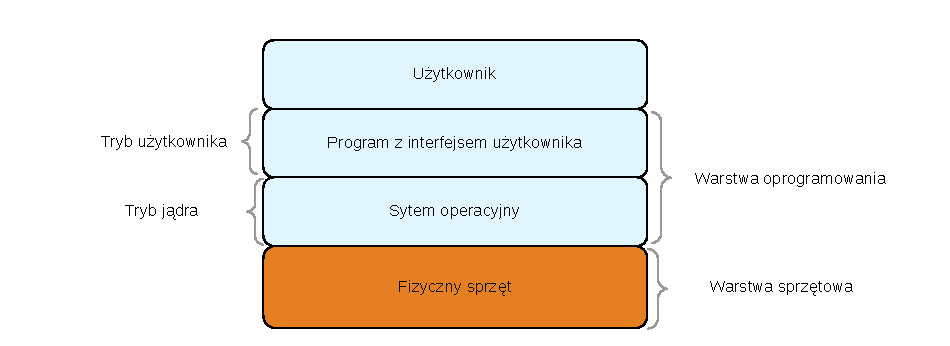
\includegraphics[width=0.8\textwidth]{img/Rysunek1.pdf}
    \caption{Warstwowy model systemu komputerowego}
    \label{fig:rysunek1}
\end{figure}

Jak pokazano na schemacie, najniższy poziom stanowi warstwa sprzętowa, do której zalicza się wszystkie fizyczne komponenty urządzenia,
takie jak \textbf{jednostka centralna} (ang. \textit{Central Processing Unit}, CPU), \textbf{pamięć} oraz \textbf{urządzenia wejścia-wyjścia} (ang. \textit{Input/Output Devices}, I/O). 
Ponad nią znajduje się warstwa oprogramowania, na którą składa się zarówno system operacyjny, jak i programy użytkownika. 
Choć oba te elementy należą do tej samej warstwy, funkcjonują one na innych zasadach. Odróżnia je praca w różnych trybach procesora, różniących się poziomem uprawnień oraz zakresem dostępu do fizycznych urządzeń.
Tryby te nazywają się odpowiednio \textbf{trybem jądra} (ang. \textit{kernel mode}), dla systemu operacyjnego, oraz \textbf{trybem użytkownika} (ang. \textit{user mode}), dla aplikacji użytkownika. 
Szczegółowa omównienie przytoczonych trybów oraz mechanizmów ich przełączania zostanie omówiona w dalszych częściach tego rozdziału.

Warto przy tym podkreślić, że w przytoczonej pozycji literatury \cite{Abraham_Silberschatz} jako integralny komponent struktury systemu komputegowego uwzględnia się jego użytkownika. 
Zabieg ten ma na celu jednoznaczne wskazanie, że przy projektowaniu dowolnego systemu komputerowego należy zawsze pamiętać o jego ostatecznym przeznaczeniu oraz o użytkowniku końcowym.

W modelu warstwowym architektury komputerowej system operacyjny pełni szczególną rolę, zarządzając granicą między aplikacjami a warstwą fizyczną. W celu zapewnienia poprawnego i przewidywalnego działania systemu wprowadza poziomy abstrakcji, które są niezbędne z kilku istotnych powodów:

\begin{enumerate}
\item \textbf{Konieczność zapewnienia bezpieczeństwa } - Współczesne systemy operacyjne charakteryzują się ogromną złożonością, a ich kod źródłowy sięga kilkudziesięciu milionów linii \cite{Tanenbaum}.
 Izolacja poszczególnych poziomów wprowadza wyraźną hierarchię uprawnień. Dzięki temu błąd powstały w kodzie aplikacyjnym pozostaje odizolowany i nie wpływa bezpośrednio na stabilność pozostałych funkcjonalności systemowych ani na pracę samego sprzętu.
\item \textbf{Zapewnienie przenoszalności oprogramowania} - Zastosowanie warstw pośrednich sprawia, że oprogramowanie nie jest bezpośrednio uzależnione od konkretnych urządzeń fizycznych. Pozwala to na uruchamianie tych samych programów na różnorodnych platformach sprzętowych,
 umożliwiając przy tym niezależny rozwój warstwy aplikacyjnej i sprzętowej.
\item \textbf{Umożliwienie korzystania z narzędzi wysokiego poziomu} - Ukrycie technicznych szczegółów pracy ze sterownikami lub rejestrami pozwala na tworzenie kodu w językach wysokiego poziomu. Programista może skupić się na logice i strukturze zgodnej ze sposobem myślenia człowieka, zamiast na bezpośredniej, niskopoziomowej obsłudze układów elektronicznych.
\end{enumerate}
\section{Kluczowe abstrakcje i mechanizmy stosowane w systemach operacyjnych}
Pomimo dużej różnorodności współczesnych systemów operacyjnych, ich architektura opiera się na spójnym zestawie uniwersalnych abstrakcji i mechanizmów. Od strony koncepcyjnej rozwiązania te wprowadzają ład w złożonym środowisku sprzętowym, przybliżając sposób funkcjonowania komputera do logiki myślenia i pracy człowieka. 

Koncepcje opisane w prezentowanej sekcji pozwalają na stworzenie przejrzystego i uporządkowanego modelu zarządzania zasobami w systemie operacyjnym. 
Zrozumienie tych bazowych koncepcji jest kluczowe dla analizy wydajności, ponieważ to one determinują sposób, w jaki program aplikacji, stworznej przez użytkownika, jest uruchamiany i wykonywany na fizycznym sprzęcie.

Na potrzeby niniejszej pracy konieczne jest przedstawienie następujących pojęć i mechanimów:
\begin{itemize}
    \item  \textbf{Tryby pracy procesora}
    \item \textbf{Proces}
    \item  \textbf{Wątek}
    \item \textbf{Szeregowanie zadań}
    \item \textbf{Pamięć wirtualna}
    \item \textbf{Mechanizmy synchronizacji i współbieżności}
\end{itemize}
\subsection{Tryby pracy procesora}
Współczesne komputery realizują ochronę zasobów poprzez tryby pracy procesora \cite{Abraham_Silberschatz}, z których kluczowe to \textbf{tryb użytkownika} (ang. user mode) oraz \textbf{tryb jądra} (ang. kernel mode). Aplikacje użytkownika funkcjonują w trybie użytkownika, nieuprzywilejowanym, co uniemożliwia im między innymi, bezpośredni dostęp do urządzeń peryferyjnych oraz fizycznej pamięci.

Wszelkie operacje wymagające kontroli nad sprzętem realizowane są za pośrednictwem \textbf{wywołań systemowych} \cite{Abraham_Silberschatz} (ang. system calls), które przełączają procesor w uprzywilejowany tryb jądra.

\subsection{Procesy}
\textbf{Proces} (ang. \textit{process}) można rozumieć jako wykonujący się program komputerowy \cite{Abraham_Silberschatz}.Jego kluczową cechą jest przydzielona, odizolowana od innych procesów wirtualna \textbf{przestrzeń adresowa}
Jej wprowadzenie ma zagwarantować bezpieczeństwo – błąd w obrębie jednego procesu nie wpływa bezpośrednio na stabilność procesów systemowych i innych procesów użytkownika.  

Współczesne systemy komputerowe składają się z licznych komponentów i aplikacji, co sprawia, że na wspólnych, fizycznych zasobach sprzętowych funkcjonuje jednocześnie wiele procesów. 
Ze względu na to, że pojedynczy rdzeń procesora może w danej chwili realizować tylko jedno zadanie, system operacyjny stosuje przełączanie kontekstu, cyklicznie przydzielając czas procesora poszczególnym procesom.
Ponieważ każdy proces operuje w odrębnej przestrzeni adresowej, zmiana ta wymaga przeładowania pamięci operacyjnej. 
W efekcie przełączanie kontekstu między procesami jest operacją stosunkowo czasochłonną i wiąże się z zauważalnym opóźnieniem, które można nazywać też \textbf{narzutem systemu operacyjnego} \cite{Tanenbaum}.

\subsection{Wątki}
\textbf{Wątek} (ang. \textit{thread}) stanowi wyodrębnioną jednostkę wykonawczą (ciąg instrukcji) uruchamianą na procesorze, funkcjonującą w obrębie konkretnego procesie \cite{Tanenbaum}. 

W ramach jednego procesu może działać wiele wątków wykonujących się we wspólnej przestrzeni adresowej. Wątki należące do tego samego procesu współdzielą ze sobą zasoby systemowe (m.in. przestrzeń adresową, zmienne globalne czy otwarte pliki), jednak każdy z nich posiada własny, prywatny kontekst wykonania \cite{Tanenbaum}, na który składają się:
\begin{itemize}
    \item \textbf{Licznik instrukcji} (ang. \textit{Program Counter}),
    \item \textbf{Zestaw rejestrów procesora},
    \item \textbf{Prywatny stos} (przechowujący zmienne lokalne oraz historię wywołań funkcji),
    \item \textbf{Stan wątku} (np. uruchomiony, zablokowany, gotowy).
\end{itemize}
Dzięki współdzieleniu przestrzeni adresowej wątki generują znacznie mniejszy narzut czasowy niż procesy, przy przełączaniu, wymagając jednak stosowania odpowiednich mechanizmów synchronizacji.

Zarządzanie wątkami może być realizowane w przestrzeni użytkownika lub bezpośrednio w jądrze systemu.
W celu zapewnienia przenoszalności oprogramowania wielowątkowego między różnymi środowiskami operacyjnymi stworzony został standard \textbf{POSIX Threads} (znany jako \textbf{Pthreads}, zdefiniowany w normie IEEE 1003.1c) \cite{Tanenbaum}. Definiuje on uniwersalne interfejsy programistyczne przeznaczone m.in. do tworzenia, kończenia oraz synchronizacji pracy wątków.

\subsection{Szeregowanie zadań}
\textbf{Szeregowanie zadań} odpowiada za zarządzanie przydziałem czasu procesora. Ponieważ pojedynczy rdzeń CPU nie może wykonywać wielu zadań jednocześnie, \textbf{planista} (ang. \textit{scheduler}) decyduje o kolejności i czasie uruchamiania wątków i procesów na podstawie określonych algorytmów \cite{Abraham_Silberschatz}.
Mechanizm ten zapewnia sprawiedliwy dostęp do zasobów i płynność działania systemu, jednak częsta zmiana wykonywanych zadań generuje bezpośredni narzut czasowy związany z przełączaniem kontekstu. 
\subsection{Pamięć wirtualna}
\textbf{Pamięć wirtualna} sprawia, że procesy nie operują bezpośrednio na fizycznej pamięci operacyjnej, lecz na wirtualnej przestrzeni adresowej przydzielanej i mapowanej na sprzęt przez \textbf{jednostkę zarzadzania pamiecia (MMU (ang. \textit{Memory Management Unit}) )}\cite{Tanenbaum}.

W kontekście pamięci wirtualnej kluczowym mechanizmem jest \textbf{stronnicowanie} \cite{Tanenbaum}. Polega ono na podziale wirtualnej przestrzeni adresowej programu na bloki o stałym rozmiarze, zwane stronami (ang. \textit{pages}), które są dynamicznie odwzorowywane na fizyczną pamięć operacyjną. Operacje tę wykonuje jednostka MMU.
Mechanmizm zarządzania pamięcią wirtualną zostało opisane, na przykładzie systemu Linux w sekcji \ref{Linux_wykorzystaniePamieci}

\subsection{Mechanizmy synchronizacji i współbieżności}


\section{Systemy wbudowane czasu rzeczywistego wraz z ich podziałem}
Systemem wbudowanym nazywamy dedykowany system komputerowy, który stanowi integralną część większego urządzenia lub maszyny i jest zaprojektowany do wykonywania 
ściśle określonego zadania \cite{Tanenbaum}. W przeciwieństwie do komputerów ogólnego przeznaczenia (takich jak komputery osobiste czy smartfony), 
na których użytkownik może uruchamiać dowolne aplikacje, system wbudowany ma z góry zdefiniowaną funkcję i nie jest przeznaczony do późniejszych, swobodnych modyfikacji przez użytkownika końcowego.

Szczególną grupą w obrębie systemów wbudowanych są \textbf{systemy wbudowane czasu rzeczywistego}. Są to takie systemy, których poprawność wyniku prztwarzania nie zależy tylko od poprawności logicznej odpowiedzi, ale też od czasu przetwarzania, poprzedzającego odpowiedź systemu \cite{WangK}.
W przypadku niewypracowania odpowiedzi w zadanym czasie zdarzenie to jest traktowane jako błąd systemu, co w skrajnych przypadkach może prowadzić do awarii lub uszkodzenia fizycznego sprzętu. 

Systemy czasu rzeczywistego są powszechnie stosowane w zastosowaniach krytycznych, takich jak przemysł zbrojeniowy, aparatura medyczna czy branża motoryzacyjna, co wymusza wprowadzenie ścisłych kryteriów oceny ich niezawodności. W celu jednoznacznego zdefiniowania wymagań dotyczących determinizmu czasowego,
 w literaturze wprowadza się klasyfikacje systemów ze względu na rygor zachowania narzuconych terminów.
W literaturze \cite{Tanenbaum} systemy czasu rzeczywistego dzieli się na:
\begin{itemize}
    \item \textbf{Systemy twarde (Hard real-time systems )} 
    \item \textbf{Systemy miękkie (Soft real-time systems )}
    \item \textbf{Systemy stabilne (Firm real-time systems )} 
\end{itemize}
W celu lepszego zobrazowania podzialu systmów czasu rzeczywistego, na rysunku \cref{fig:wykresy RTOS} przedstawiono wykresy funkcji przydatności odpowiedzi $y(t)$ od czasu jej wypracowania przez system \cite{Tanenbaum}. 
\begin{figure}[htbp]
\centering
\definecolor{userblue}{RGB}{225, 243, 254}

% --- RZĄD GÓRNY: RYSUNKI A ORAZ B (ZBLIŻONE DO SIEBIE) ---
\begin{subfigure}[b]{0.42\textwidth}
\centering
\begin{tikzpicture}[>=stealth, scale=0.6, every node/.style={transform shape}]
\fill[userblue] (-1,-1) rectangle (7.5,4.2);
\draw[->, thick] (-0.5,0) -- (7,0) node[right=3pt, font=\large] {$t$};
\draw[->, thick] (0,-0.8) -- (0,4) node[right=3pt, font=\large] {$y(t)$};
\draw[ultra thick] (1,2.8) -- (3,2.8) -- (5,0) -- (6.8,0); 
\draw[dotted, thick] (0,2.8) -- (1,2.8);   
\draw[dotted, thick] (1,0) -- (1,2.8); 
\draw[dotted, thick] (3,0) -- (3,2.8); 
\node[below, font=\large] at (1,0) {$t_0$};
\node[below, font=\large] at (3,0) {$t_1$};
\node[below, font=\large] at (5,0) {$t_T$};
\node[left=3pt, font=\large] at (0,2.8) {$u$};
\node[left=3pt, font=\large] at (0,0) {$0$};
\node[draw=black, thin, fill=white, inner sep=1pt, anchor=north east, font=\scriptsize] at (6.8, 3.9) {
    $\displaystyle y(t) = 
    \begin{cases}
    u & t_0 < t < t_1 \\
    u \frac{t_T - t}{t_T - t_1} & t_1 < t < t_T \\
    0 & t \ge t_T
    \end{cases}$
};
\end{tikzpicture}
\caption{Miękki system czasu rzeczywistego}
\label{fig:softRTOS wykres}
\end{subfigure}
\quad 
\begin{subfigure}[b]{0.42\textwidth}
\centering
\begin{tikzpicture}[>=stealth, scale=0.6, every node/.style={transform shape}]
\fill[userblue] (-1,-1) rectangle (7.5,4.2);
\draw[->, thick] (-0.5,0) -- (7,0) node[right=3pt, font=\large] {$t$};
\draw[->, thick] (0,-0.8) -- (0,4) node[right=3pt, font=\large] {$y(t)$};
\draw[ultra thick] (1,2.8) -- (4.5,2.8); 
\draw[ultra thick, dashed] (4.5,2.8) -- (4.5,0); 
\draw[ultra thick] (4.5,0) -- (6.8,0);
\draw[dotted, thick] (0,2.8) -- (1,2.8);   
\draw[dotted, thick] (1,0) -- (1,2.8); 
\node[below, font=\large] at (1,0) {$t_0$};
\node[below, font=\large] at (4.5,0) {$t_T$};
\node[left=3pt, font=\large] at (0,2.8) {$u$};
\node[left=3pt, font=\large] at (0,0) {$0$};
\node[draw=black, thin, fill=white, inner sep=1pt, anchor=north east, font=\scriptsize] at (6.8, 3.9) {
    $\displaystyle y(t) = 
    \begin{cases}
    u & t_0 < t < t_T \\
    0 & t \ge t_T
    \end{cases}$
};
\end{tikzpicture}
\caption{Solidny system czasu rzeczywistego}
\label{fig:firm RTOS wykres}
\end{subfigure}

\vspace{6ex} % Zdecydowanie większy odstęp pionowy

% --- RZĄD DOLNY: RYSUNEK C NA PEŁNĄ SZEROKOŚĆ (CENTROWANY DO STRONY) ---
\begin{subfigure}[b]{\textwidth}
\centering
\begin{tikzpicture}[>=stealth, scale=0.6, every node/.style={transform shape}]
% 1. Kolor tła
\fill[userblue] (-1,-3.5) rectangle (7.5,4.2);
% 2. Osie
\draw[->, thick] (-0.5,0) -- (7,0) node[right=3pt, font=\large] {$t$};
\draw[->, thick] (0,-3.2) -- (0,4) node[right=3pt, font=\large] {$y(t)$};
% 3. Główna linia wykresu
\draw[ultra thick] (1,2.8) -- (4.5,2.8); 
\draw[ultra thick, ->, dashed] (4.5,2.8) -- (4.5,-2.8); 
% 4. Linie pomocnicze
\draw[dotted, thick] (0,2.8) -- (1,2.8);   
\draw[dotted, thick] (1,0) -- (1,2.8); 
% 5. Etykiety
\node[below, font=\large] at (1,0) {$t_0$};
\node[below, font=\large] at (4.5,0) {$t_T$};
\node[left=3pt, font=\large] at (0,2.8) {$u$};
\node[left=3pt, font=\large] at (0,-2.8) {$-\infty$};
% 6. Wzór
\node[draw=black, thin, fill=white, inner sep=1pt, anchor=north east, font=\scriptsize] at (6.8, 3.9) {
    $\displaystyle y(t) = 
    \begin{cases}
    u       & t_0 < t < t_T \\
    -\infty & t \ge t_T
    \end{cases}$
};
\end{tikzpicture}
\caption{Twardy system czasu rzeczywistego}
\label{fig:Hard RTOS wykres}
\end{subfigure}

\caption{Zestawienie przebiegów funkcji przydatności odpowiedzi $y(t)$ w dziedzinie czasu \cite{Tanenbaum}.}
\label{fig:wykresy RTOS}
\end{figure}

Przed przystąpieniem do analizy poszczególnych wykresów, konieczne jest zdefiniowanie parametrów oraz skrótów stanowiących zmienne opisujące te funkcje:
\begin{itemize}
    \item $t$ -- oś czasu, reprezentująca moment dostarczenia odpowiedzi przez system,
    \item $y(t)$ -- funkcja przydatności (wartości) odpowiedzi dla obsługiwanego procesu,
    \item $u$ -- maksymalna, nominalna przydatność prawidłowo wypracowanego wyniku,
    \item $t_0$ -- moment pojawienia się zdarzenia lub żądania wypracowania odpowiedzi przez system,
    \item $t_1$ -- czas graniczny, do którego odpowiedź zachowuje pełną wartość (w systemach miękkich),
    \item $t_T$ -- ostateczny limit czasowy (ang. \textit{deadline}), po przekroczeniu którego odpowiedź nie ma już pełnej wartości.
\end{itemize}
Analizując przebiegi funkcji przydatności dla poszczególnych klas systemów, można precyzyjnie scharakteryzować ich zachowanie.

Najbardziej restrykcyjne kryteria czasowe są charkerystyczne dla twardych systemy czasu rzeczywistego, co zobrazowano na rysunku \ref{fig:Hard RTOS wykres}.
Ich stosowanie gwarantuje bezwzględnie terminowe wypełnienie zadań krytycznych przed upływem limitu $t_T$. Przekroczenie czasu przetwarzania powoduje natychmiastowy spadek funkcji przydatności do wartości $-\infty$.
W przypadku rozwiązań spóźniona odpowiedź jest nie tylko całkowicie bezużyteczna, ale jej pojawienie się po wyznaczonym terminie jest najczęściej równoznaczne z wystąpieniem krytycznego błędu, który może doprowadzić do poważnej awarii lub fizycznego uszkodzenia całego systemu.

Kolejną z omawianych grup stanowią miękkie systemy czasu rzeczywistego, których zachowanie zilustrowano na rysunku \ref{fig:softRTOS wykres}. Systemy te cechują się mniejszym rygorem w kwestii terminowości, co oznacza, że zadania są wykonywane tak szybko, 
jak to możliwe, a ewentualne opóźnienia nie niosą za sobą skutków katastrofalnych. Jeśli odpowiedź zostanie dostarczona po czasie $t_1$, ale przed ostatecznym limitem $t_T$, jej przydatność maleje, powodując jedynie spadek jej jakości.
Przy przetwarzaniu przekracającym czas $t_T$ przydatność odpowiedzi wynosi zero. 

Solidne systemy czasu rzeczywistego stanowią pewnego rodzaju kompromis pomięczy twardymi, a miękkimi systemamu czasu rzeczywistego. Zachowanie funkcji przydatności systemów solidnych przedstawiono na rysunku \ref{fig:firm RTOS wykres}. 
Każda odpowiedź dostarczona w przedziale od $t_0$ do $t_T$ zachowuje stałą, pełną wartość $u$. W momencie przekroczenia terminu granicznego $t_T$ przydatność wyniku natychmiastowo i skokowo spada do zera.
Choć fakt spóźnienia powoduje całkowitą nieprzydatność rozwiązania, to sytuacja ta wciąż nie generuje bezpośredniego zagrożenia dla stabilności czy integralności samego systemu. 

Zdefiniowane powyżej rygory czasowe określają, teoretyczny oczekiwania wobec systemu czasu rzeczywistego. W praktyce realizacja tych założeń sprowadza się do oceny zasadności stosowania \textbf{systemu operacyjnego czasu rzeczywistego} 
w zderzeniu z bezpośrednim programowaniem sprzętu. Decyzja ta bezpośrednio determinuje strukturę i elastyczność budowanego środowiska.


\section{Architektura struktur jądra systemów operacyjnych}

Systemy operacyjne można klasyfikować według wielu kryteriów, z których jednym z najczęsciej spotykanym jest podział, ze względu na ich docelowe przeznaczenie. Przy takim podziale możemy wyróżnić systemy operacyjne generalnego przeznaczenia, systemy operacyjne rozproszone, systemy operacyjne komputerów nmainframe, systemy operacyjne serwerów oraz wiele innych \cite{Tanenbaum}.

Jednakże, w kontekście analizy wydajności kluczowy jest podział ze względu na strukturę systemu, która określa architekturę jego jądra.  Na tym etapie jądro systemu możemy zdefiniować jedyny program, który działa w pamięci komputera nieprzerwanie przez cały czas od jego uruchomienia, pełniąc funkcję pomostu komunikacyjnego między uruchomionymi aplikacjami,
a fizycznym sprzętem \cite{Abraham_Silberschatz}.

Konstrukcja jądra decyduje o sposobie komunikacji między usługami systemowymi, a warstwą aplikacyjną, co bezpośrednio wpływa na narzuty czasowe oraz efektywność optymalizacji kodu programów. 
Z uwagi na to, że przedmiotem badań w niniejszej pracy jest system Linux, analiza skupi się głównie na architekturze monolitycznej. Dla celów porównawczych zostanie ona zestawiona z inną szeroko spotykaną architekturą w systemach wbudowanych - strukturą mikrojądra.

W \textbf{architekturze monolitycznej} (ang. \textit{monolithic kernel}) wszystkie główne zadania systemu operacyjnego są połączone w jeden rozbudowany program komputerowy \cite{Tanenbaum}. Zarządzanie pamięcią, programami oraz wszystkimi sterownikami urządzeń odbywa się we wspólnej przestrzeni.
Takie podejście sprawia, że jądro zawiera w sobie ogromną liczbę elementów, co mocno komplikuje proces jego tworzenia oraz późniejszego szukania błędów. Największą zaletą architektury monolitycznej jest jednak wysoka prędkość przetwarzania informacji -- z uwagi na to, że 
jądro jest w całości kompilowane do jednego programu, poszczególne funkcjonalności mogą z siebie nawzajem korzystać, co znacząco przyśpiesza działanie systemu. 
Przy architekturze monolitycznej aplikacje użytkownika są uruchamiane jako osobne procesy w chronionej pamięci. Dzięki temu jądro nie jest narażone na błędy w programach użytkownika, a różne aplikacje nie mogą nawzajem bezpośrednio mieć dostępu zasobów im nie przydzielonych.
Główną wadą systemów monolitycznych pozostaje jednak słaba odporność na awarie samego jądra; jeśli błąd pojawi się w jego obrębie niego, na przykład w jednym ze sterowników, może dojść do awarii całego systemu.

\textbf{Architektura mikrojądra} (ang. \textit{microkernel}) opiera się na zasadzie minimalizacji kodu wykonywanego z najwyższymi uprawnieniami procesora \cite{Abraham_Silberschatz}. Kompletny system operacyjny składa się w tym przypadku z uproszczonego jądra
oraz zestawu współpracujących ze sobą procesów systemowych. Samo mikrojądro realizuje jedynie fundamentalne zadania, takie jak zarządzanie wątkami oraz obsługa komunikacji międzyprocesowej \cite{Tanenbaum}. Wszystkie pozostałe usługi, wliczając w to sterowniki urządzeń i systemy plików, są odseparowane od jądra i funkcjonują jako niezależne programy w przestrzeni użytkownika.

Główną zaletą takiego podejścia jest wysoka stabilność środowiska -- awaria oprogramowania lub sterownika nie narusza integralności samego jądra. System potrafi zrestartować uszkodzony proces bez zaburzania pracy całego systemu. 
Wadą tego rozwiązania jest jednak niższa wydajność, wynikająca z narzutu czasowego na ciągłą konieczność komunikacji międzyprocesowej oraz częste przełączanie kontekstu procesora.

\section{Studium przypadku systemu operacyjnego Linux}
System operacyjny Linux wywodzi się z  tradycji architektonicznej rodziny systemów "Unix", czerpiąc z niej kluczowe założenia projektowe, takie jak wielozadaniowość, wielodostępność oraz podział przestrzeni pamięci \cite{Tanenbaum}. Jego rozwój rozpoczął się w 1991 roku z inicjatywy Linusa Torvaldsa, a dziś stanowi on jeden z najważniejszych i najczęściej wykorzystywanych projektów tworzonych w modelu otwartego oprogramowania ( ang.\textit{open source}) \cite{Tanenbaum}.
Dzięki wsparciu globalnej społeczności Linux stał się najczęściej wykorzystywanym systemem komputerowym w wielu zastosowaniach, począwszy od  infrastruktury serwerowej przez systemy wbudowane, aż po chmury obliczeniowe.

Z perspektywy użytkownika klasycznym i wysoce elastycznym sposobem komunikacji z systemem Linux  jest powłoka (ang. \textit{shell}), w systemach Linux reprezentowana najczęściej przez program \textit{bash} \cite{Tanenbaum}. Z technicznego punktu widzenia jest to zwykły program działający w przestrzeni użytkownika, który pełni rolę interpretera poleceń \cite{Tanenbaum}. Powłoka pozwala na uruchamianie innych programów wraz z odpowiednimi parametrami.
Do jej kluczowych funkcjonalności należy elastyczne przekierowywanie standardowych strumieni wejścia i wyjścia oraz łączenie pojedynczych programów w potoki (ang. \textit{pipelines}), co pozwala na przekazywanie wyników między różnymi procesami \cite{Tanenbaum}.
Ponadto powłoka umożliwia asynchroniczne uruchamianie zadań w tle oraz tworzenie skryptów, które dzięki obsłudze zmiennych i instrukcji sterujących (np. pętli czy instrukcji warunkowych) pozwalają na automatyzację złożonych operacji systemowych \cite{Abraham_Silberschatz}.

Kluczowym elementem systemu jest jądro o strukturze monolitycznej \cite{LinuxKernelDevelopment}, które odpowiada za bezpośrednią kontrolę nad najważniejszymi zasobami systemu.
Z uwagi na tę architekturę oraz konieczność zapewnienia bezpieczeństwa, aplikacje działające w przestrzeni użytkownika nie mają bezpośredniego dostępu do krytycznych zasobów systemu. Wszelka interakcja z zasobami zarządzanymi przez system musi odbywać się za pośrednictwem zdefiniowanego interfejsu wywołań systemowych, który w systemie Linux jest zgodny ze standardem \textbf{POSIX} \cite{Tanenbaum}. Każde takie wywołanie wymusza sprzętowe przełączenie procesora do trybu jądra. Operacja ta wymaga zapisania  stanu rejestrów oraz zmiany kontekstu wykonania, co  wiąże się z dodatkowym narzutem czasowym.
\subsection{Procesy, wątki w systemie Linux}

W przeciwieństwie do wielu innych systemów operacyjnych, Linux nie wprowadza ścisłego, wewnętrznego rozróżnienia między procesami, a wątkami\cite{Tanenbaum}. Każdy kontekst wykonania, niezależnie od tego, czy jest to jednowątkowy proces, czy jeden z wielu wątków wewnątrz procesu, jest reprezentowany w jądrze jako zadanie (ang. \textit{task}) za pomocą struktury danych \texttt{task\_struct} \cite{LinuxKernelDevelopment}. 

Klasyczne tworzenie nowego procesu odbywa się poprzez wywołanie systemowe \texttt{fork}. Aby uniknąć kosztownego i nieefektywnego kopiowania całej pamięci, Linux stosuje optymalizację kopiowania przy zapisie (ang. \textit{copy on write})\cite{LinuxKernelDevelopment}. Początkowo proces potomny otrzymuje własne tablice stron, jednak wskazują one na fizyczne strony pamięci procesu macierzystego z atrybutem tylko do odczytu. Nowa kopia strony jest alokowana w pamięci RAM dopiero w momencie, gdy któryś z procesów spróbuje dokonać na niej operacji zapisu \cite{Tanenbaum}.

Z kolei fundamentalną różnicą w architekturze Linuksa, w porównaniu do klasycznych systemów UNIX, jest obsługa wątków. Wprowadzono w nim wywołanie systemowe \texttt{clone}, które zaciera tradycyjną różnicę między procesami a wątkami \cite{Tanenbaum}, umożliwiając tworzenie nowego wątku z bardzo podobnymi cechami do klasycznego procesu. 

Pozwala ono zminimalizować narzut systemowy poprzez precyzyjne sterowanie tym, co jest kopiowane, a co współdzielone. Wywołanie to przyjmuje jako argument mapę bitową, w której poszczególne flagi (np. \texttt{CLONE\_FILES}, \texttt{CLONE\_SIGHAND}) decydują o współdzieleniu deskryptorów plików czy tablicy obsługi sygnałów \cite{Tanenbaum}.
\subsection{Szeregowanie i synchronizacja w systemie Linux}
System operacyjny Linux posiada przemyślany i wysoce elastyczny mechanizm szeregowania zadań oraz synchronizacji, który obsługuje zarówno standardowe programy użytkowe, jak i zadania czasu rzeczywistego \cite{Tanenbaum}. 

W kontekście planowania czasu procesora, jądro wyróżnia trzy główne klasy wątków: zadania czasu rzeczywistego typu FIFO, zadania czasu rzeczywistego z rotacją (ang. \textit{round-robin}) oraz zadania standardowe \cite{Tanenbaum}. Wątki czasu rzeczywistego otrzymują zawsze najwyższe priorytety (w skali od 0 do 99). Mimo swojej nazwy nie dają one ścisłych gwarancji dotrzymania terminów (ang. \textit{deadlines}), a jedynie zapewniają bezwzględne pierwszeństwo wykonania przed zwykłymi aplikacjami, \cite{Tanenbaum}. Jest to bardzo istotna cecha systemu Linux, która pokazuje, że nie jest on odpowiedni (w klasycznej, nieprzerobionej wersji systemu) do bezpośredniego wykorzystania w twardych systemach czasu rzeczywistego \cite{LinuxKernelDevelopment}.
Wątki typu FIFO działają aż do momentu dobrowolnego oddania procesora lub wywłaszczenia przez zadanie o wyższym priorytecie, podczas gdy wątkom szeregowanym cyklicznie przydzielane są dodatkowo określone kwanty czasu \cite{Tanenbaum}.

Z kolei standardowe zadania o niższych priorytetach (od 100 do 139) są z reguły obsługiwane przez algorytm \textit{Completely Fair Scheduler} (CFS) \cite{Tanenbaum}, który optymalizuje i sprawiedliwie rozdziela czas procesora z wykorzystaniem struktury drzewa czerwono-czarnego \cite{Abraham_Silberschatz}.

Uzupełnieniem efektywnego zarządzania zadaniami są zróżnicowane mechanizmy synchronizacji, które zastąpiły historyczną, nieefektywną globalną blokadę jądra. Aby zminimalizować ryzyko konfliktów o dostęp do zasobów, Linux udostępnia pełen przekrój rozwiązań: od operacji atomowych i barier pamięci, poprzez blokady wirujące (ang. \textit{spinlocks}) \cite{LinuxKernelDevelopment} – optymalne, gdy wątek nie powinien być usypiany – aż po wysokopoziomowe muteksy i semafory dla zadań mogących bezpiecznie przejść w stan oczekiwania \cite{Tanenbaum}.
\subsection{Zarządzanie pamiecią}\label{Linux_wykorzystaniePamieci}

W systemie Linux pamięć jest stronnicowana. W związku z tym, podstawową jednostką do zarządzania pamięcią fizyczną jest struktura o nazwie \textit{page} \cite{LinuxKernelDevelopment}. Z uwagi na ograniczenia sprzętowe niektórych architektur, pamięć fizyczna została logicznie podzielona na strefy (ang. \textit{zones}). Należą do nich między innymi \texttt{ZONE\_DMA}, przeznaczona na operacje bezpośredniego dostępu do pamięci, \texttt{ZONE\_NORMAL}, zawierająca standardowe strony, oraz \texttt{ZONE\_HIGHMEM} \cite{Tanenbaum}. 

Każdy proces uruchomiony w systemie operuje na własnej wirtualnej przestrzeni adresowej, która logicznie dzieli się na trzy główne segmenty: kod, dane oraz stos \cite{Tanenbaum}. Segment kodu przechowuje instrukcje programu i domyślnie posiada atrybut umożliwiający jedynie jego odczyt, co pozwala na bezpieczne współdzielenie go między wieloma jednoczesnymi uruchomieniami tego samego programu \cite{Abraham_Silberschatz}. Segment danych przechowuje zmienne globalne i statyczne, przy czym dla zmiennych niezainicjowanych  Linux stosuje optymalizację: mapuje je na jedną fizyczną, wyzerowaną stronę, dopóki proces nie spróbuje dokonać modyfikacji, co wyzwala mechanizm kopiowania przy zapisie (ang. \textit{copy-on-write}) \cite{Tanenbaum}. Ponadto jądro oferuje mechanizm mapowania plików w pamięci, co umożliwia procesom bezpośredni dostęp do danych plikowych lub współdzielonych bibliotek z pominięciem standardowych wywołań systemowych \cite{Tanenbaum}.

Do zarządzania przydziałem fizycznych stron pamięci Linux wykorzystuje \textbf{algorytm bliźniaków} (ang. \textit{buddy algorithm}) \cite{Tanenbaum}. Choć mechanizm ten jest w większości przypadków wysoce wydajny, może prowadzić do zjawiska fragmentacji wewnętrznej w przypadku konieczności alokacji struktur o rozmiarach znacznie mniejszych niż domyślne wielkości strony. Aby zminimalizować ten problem i zredukować narzut systemowy, system wdraża mechanizm dyspozytora płytowego (ang. \textit{slab allocator}) \cite{LinuxKernelDevelopment}, który działa dysponuje pamiecia poprzez algorytm blizniakow, aby pozniej podzieli strone na mniejsze fragmenty i umozliwic jej zarzadzanie \cite{Tanenbaum}. 

Na poziomie interfejsu programistycznego jądra alokacja pamięci odbywa się za pomocą kilku wyspecjalizowanych funkcji do zarządzania pamięcią.Warto tutaj wspominieć o tych najpowszechniejszych, czyli \texttt{kmalloc}, gwarantująca przydział obszaru ciągłego zarówno w przestrzeni wirtualnej, jak i fizycznej \cite{LinuxKernelDevelopment} oraz \texttt{vmalloc} wykorzystywana do alokacji większych struktur, niewymagających ciągłości fizycznej. Ta druga jednak wiąże się  z  większym narzutem wydajnościowym wynikającym z konieczności modyfikacji tablic stron \cite{LinuxKernelDevelopment}.
\chapter{Wybrany algorytm przetwarzania danych i techniki optymalizacji programów komputerowych}
\section{Opis i analiza Szybkiej Transformaty Fouriera}
\subsection{Podstawy matematyczne algorytmu FFT}
\textbf{Przekształcenie Fouriera} (ang. \textit{Fourier Transform}) dla sygnałów ciągłych służy do wyznaczania widma częstotliwościowego $X(j\omega)$ sygnału czasu ciągłego $x(t)$ \cite{ZielinskiDSP}. Wzory przekształcenia prostego i odwrotnego definiuje się następująco \cite{ZielinskiDSP}:

\begin{equation}
X(j\omega) = \int_{-\infty}^{\infty} x(t)\, e^{-j\omega t}\, dt,
\qquad
x(t) = \frac{1}{2\pi}\int_{-\infty}^{\infty} X(j\omega)\, e^{j\omega t}\, d\omega
\end{equation}

gdzie $\omega = 2\pi f$ oznacza pulsację, a $f$ częstotliwość wyrażoną w hercach.

Aby całka określająca $X(j\omega)$ była zbieżna, sygnał $x(t)$ musi spełniać tzw. \textbf{warunki Dirichleta}: być bezwzględnie całkowalny, mieć skończoną liczbę ekstremów oraz skończoną liczbę punktów nieciągłości w dowolnym skończonym przedziale \cite{ZielinskiDSP}.

Matematyczne podstawy ciągłej transformaty Fouriera są jednak nie do końca przydatne w świecie cyfrowego przetwarzania sygnałów, właśnie z uwagi na fakt, że sygnały, na których pracują maszyny cyfrowe, są dyskretne, a nie ciągłe. W tym celu definiuje się dyskretną transformatę Fouriera, która powstaje w wyniku dyskretyzacji szeregu Fouriera dla sygnału okresowego o okresie $N$ \cite{ZielinskiDSP}.

W systemach cyfrowych przetwarzany sygnał dostępny jest w postaci skończonego ciągu próbek $x(n)$, $n = 0, 1, \dots, N-1$, pobranych z częstotliwością próbkowania $f_{pr}$. Powyższy wzór na ciągłą transformatę Fouriera nie da się więc bezpośrednio zastosować. Zamiast niego widmo sygnału wyznacza się za pomocą \textbf{dyskretnej transformacji Fouriera} (DFT, ang. \textit{Discrete Fourier Transform}). Matematyczne przekształcenia dla prostej i odwrotnej DFT definiuje się następująco \cite{ZielinskiDSP}:

\begin{equation}
X(k) = \frac{1}{N}\sum_{n=0}^{N-1} x(n)\, e^{-j\frac{2\pi}{N}kn},
\qquad k = 0, 1, \dots, N-1
\label{eq:dft_analiza}
\end{equation}

\begin{equation}
x(n) = \sum_{k=0}^{N-1} X(k)\, e^{j\frac{2\pi}{N}kn},
\qquad n = 0, 1, \dots, N-1
\end{equation}

gdzie $k$ oznacza numer składowej widma, dla której wyliczana jest aktualnie wartość transformaty. Kolejnym składowym odpowiada pulsacja $\Omega_k = 2\pi k/N$.

Wygodnym uproszczeniem powyższych zapisów jest wprowadzenie tzw. \textbf{czynnika obrotu} (ang. \textit{twiddle factor})\cite{CormenIntroductionAlgorithms}:

\begin{equation}
W_N = e^{-j\frac{2\pi}{N}}
\label{eq:twiddle}
\end{equation}

co pozwala przedstawić parę wzorów DFT w zwartej postaci \cite{ZielinskiDSP}:

\begin{equation}
X(k) = \frac{1}{N}\sum_{n=0}^{N-1} x(n)\, W_N^{kn},
\qquad k = 0, 1, \dots, N-1
\label{eq:dft_analiza_wn}
\end{equation}

\begin{equation}
x(n) = \sum_{k=0}^{N-1} X(k)\, W_N^{-kn},
\qquad n = 0, 1, \dots, N-1
\label{eq:dft_synteza_wn}
\end{equation}


W inżynierii oprogramowania do porównywania wydajności algorytmów powszechnie wykorzystuje się \textbf{notację dużego O} (ang. \textit{Big O notation}), opisującą tempo wzrostu liczby wykonywanych operacji wraz ze długości wektora przetwarzanych danych wejściowych $N$. Zapis $O(g(N))$ oznacza, że liczba wykonywanych operacji rośnie nie szybciej niż funkcja $g(N)$ pomnożona przez pewną stałą, dla odpowiednio dużych $N$ \cite{CormenIntroductionAlgorithms}.

Innymi słowy, notacja ta pomija czynniki stałe i wyrazy niższego rzędu, skupiając się na tym, jak rośnie liczba operacji wraz ze wzrostem rozmiaru danych wejściowych \cite{CormenIntroductionAlgorithms}.

Dla przykładu, bezpośrednie obliczenie wzoru \eqref{eq:dft_analiza} dla każdego z $N$ prążków widma wymaga $N$ mnożeń zespolonych, co dla całego wektora $X(k)$ wymaga wykonania zasadniczo $N^2$ mnożeń. W takim wypadku złożoność algorytmu DFT można określić jako $O(N^2)$. Przy ciągłym przetwarzaniu długich sygnałów złożoność ta stanowi istotne ograniczenie praktyczne. Jej redukcja jest możliwa dzięki zastosowaniu \textbf{algorytmu szybkiej transformacji Fouriera} (FFT, ang. \textit{Fast Fourier Transform}), który pozwala znacznie obniżyć koszt obliczeniowy.
\subsection{Szybka transformata Fouriera}
Redukcja złożoności obliczeniowej DFT jest możliwa dzięki zastosowaniu algorytmów określanych mianem szybkich transformacji Fouriera (FFT). Można w tym wypadku mówić o pewnym zbiorze rozwiązań, bazujących na tym samym koncepcie. Po raz pierwszy algorytm ten zaproponowano w latach sześćdziesiątych XX wieku w pracy \cite{CooleyTurkeyFFT}. Rodzina algorytmów FFT pozwala na znaczące obniżenie złożoności obliczeniowej, przy zachowaniu takiej samej poprawności obliczeń jak w przypadku klasycznego algorytmu DFT. FFT jest więc wydajnym sposobem na obliczenie DFT — jego złożoność obliczeniowa spada do rzędu $O(N\log_2 N)$ \cite{ZielinskiDSP}.

W pracy Cooleya-Tukeya \cite{CooleyTurkeyFFT} zaproponowano nowe podejście do obliczania dyskretnej transformaty Fouriera, polegające na rozłożeniu długiego sygnału, o $N$ próbkach, na kilka mniejszych grup. Następnie policzono transformatę osobno dla każdej z nich, by w ostatnim kroku połączyć wyniki w widmo całego sygnału.

Autorzy zauważyli również, że wybór $N$ będącego potęgą liczby 2 lub 4 jest szczególnie wygodny dla komputerów działających na liczbach binarnych. Co więcej, cały algorytm można było wykonać na tej samej tablicy danych, bez potrzeby rezerwowania dodatkowej pamięci na wyniki pośrednie \cite{CooleyTurkeyFFT}.

Zaproponowana metoda stała się inspiracją dla tworzenia kolejnych wariantów szybkiej transformaty Fouriera \cite{ZielinskiDSP}:

\begin{itemize}
    \item \textbf{Radix-2},
    \item \textbf{radix-4},
    \item \textbf{split-radix},
    \item \textbf{algorytm Gooda-Thomasa},
    \item \textbf{transformacja świergotowa (ang. \textit{chirp-Z})}.
\end{itemize}
Wszystkie realizują to samo przekształcenie, czyli dyskretną transformatę Fouriera, różnią się natomiast wewnętrznymi mechanizmami, takimi jak podejście do podziału danych czy długości pojedynczego bloku przetwarzanego sygnału \cite{ZielinskiDSP}.
Szczegółowy opis wariantów wykorzystanych w niniejszej pracy, wraz z ich implementacjami, przedstawiono w \cref{section:WariantyFFTUzyteWPracy}.

Do dalszej analizy teoretycznej posłuży popularny wariant FFT oparty na \textbf{podstawie 2} (ang. \textit{radix-2}), czyli podziale na dwa podzbiory, jako najprostszy do intuicyjnego wyjaśnienia.
Na algorytm w tej postaci składa się kilka podstawowych zagadnień, omówionych kolejno w dalszej części podrozdziału: sposób podziału danych, uporządkowanie próbek przed rozpoczęciem obliczeń oraz elementarna operacja arytmetyczna, powtarzana na każdym etapie.

Podział wektora wejściowego może być przeprowadzony na dwa podstawowe sposoby. W wariancie z \textbf{decymacją w czasie} (DIT, ang. \textit{Decimation in Time}) dzieli się próbki sygnału wejściowego na te o indeksach parzystych i nieparzystych, wykonuje DFT osobno na każdym zbiorze, a następnie odtwarza widmo całego sygnału z widm cząstkowych \cite{ZielinskiDSP}. W wariancie z \textbf{decymacją w częstotliwości} (DIF, ang. \textit{Decimation in Frequency}) postępuje się odwrotnie — dzieli się nie próbki wejściowe, lecz prążki widma wyjściowego \cite{ZielinskiDSP}.

Konsekwencją podziału jest to, że dane trafiają do obliczeń w innej kolejności niż ta pierwotna w sygnale wejściowym, więc na którymś etapie algorytmu należy je uporządkować. W algorytmach DIT robi się to na wejściu, przed właściwymi obliczeniami, i wynik otrzymuje się w kolejności naturalnej \cite{NumericalRecipesC}. W DIF jest odwrotnie — poprzestawiany jest dopiero wynik, na co zwrócono uwagę już w oryginalnej pracy \cite{CooleyTurkeyFFT}.

Samo przestawianie można wykonać na kilka różnych sposobów, z czego podstawowy polega na wielokrotnym dzieleniu próbek na parzyste i nieparzyste. Jest to jednak rozwiązanie nieefektywne, ponieważ dane sortowane są wielokrotnie \cite{ZielinskiDSP}. Okazuje się, że docelową pozycję każdej próbki da się wyznaczyć z użyciem operacji \textbf{permutacji bitowo-odwróconej} (ang. \textit{bit-reversal permutation}) \cite{CormenIntroductionAlgorithms}. Metoda ta ustawia w odwrotnej kolejności bity indeksu próbki wektora wejściowego \cite{ZielinskiDSP}, co pozwala dość niskim kosztem obliczeniowym poukładać wektor wejściowy w kolejności wymaganej przez algorytm DIT. Warto dodać, że wiele procesorów sygnałowych udostępnia sprzętowy mechanizm adresowania z odwróceniem bitów, co dodatkowo przyspiesza ten etap \cite{ZielinskiDSP}.

% ===== CLAUDE GENERATED START =====
Wynik tej operacji dla sygnału o długości $N = 16$ zestawiono w \cref{tab:bit_reversal} \cite{ZielinskiDSP}. Warto zauważyć, że w celu ponownego ustawienia próbek w pierwotnej kolejności wystarczy raz jeszcze wykonać tę samą operacje. W prezentowanej tabeli jako $n$ oznaczono indeks początkowy, a jako  $n'$ indeks po operacji bit-reversal.
\begin{table}[ht]
    \centering
    \caption{Permutacja bitowo-odwrócona indeksów próbek dla $N = 16$}
    \label{tab:bit_reversal}
    \begin{tabular}{@{}rccr@{\hspace{2.5em}}rccr@{}}
        \toprule
        $n$ & zapis dwójkowy & bity odwrócone & $n'$ &
        $n$ & zapis dwójkowy & bity odwrócone & $n'$ \\
        \midrule
        0 & \texttt{0000} & \texttt{0000} & 0  &  8  & \texttt{1000} & \texttt{0001} & 1  \\
        1 & \texttt{0001} & \texttt{1000} & 8  &  9  & \texttt{1001} & \texttt{1001} & 9  \\
        2 & \texttt{0010} & \texttt{0100} & 4  &  10 & \texttt{1010} & \texttt{0101} & 5  \\
        3 & \texttt{0011} & \texttt{1100} & 12 &  11 & \texttt{1011} & \texttt{1101} & 13 \\
        4 & \texttt{0100} & \texttt{0010} & 2  &  12 & \texttt{1100} & \texttt{0011} & 3  \\
        5 & \texttt{0101} & \texttt{1010} & 10 &  13 & \texttt{1101} & \texttt{1011} & 11 \\
        6 & \texttt{0110} & \texttt{0110} & 6  &  14 & \texttt{1110} & \texttt{0111} & 7  \\
        7 & \texttt{0111} & \texttt{1110} & 14 &  15 & \texttt{1111} & \texttt{1111} & 15 \\
        \bottomrule
    \end{tabular}
\end{table}
% ===== CLAUDE GENERATED STOP =====

Niezależnie od przyjętego wariantu uporządkowania danych, kolejną elementarną operacją wykonywaną na każdym etapie algorytmu FFT, bazujących na założeniach zaprezentowanych w \cite{CooleyTurkeyFFT}, jest tak zwana \textbf{operacja motylkowa} (ang. \textit{butterfly}) \cite{ZielinskiDSP}. Operacja ta pobiera parę liczb zespolonych $x(p)$ oraz $x(q)$, mnoży drugą z nich przez odpowiedni czynnik obrotu \eqref{eq:twiddle}, a następnie wyznacza sumę i różnicę otrzymanych w ten sposób wartości \cite{CormenIntroductionAlgorithms}:

\begin{equation}
x'(p) = x(p) + W_N^{k}\,x(q),
\qquad
x'(q) = x(p) - W_N^{k}\,x(q)
\label{eq:motylek}
\end{equation}

gdzie $p$ i $q$ oznaczają pozycje dwóch przetwarzanych elementów w tablicy danych, oddalone od siebie o połowę długości bieżącego etapu, a wykładnik $k$ — numer operacji motylkowej w obrębie tego etapu.

Istotną cechą tak zapisanej operacji jest to, że obie wartości wynikowe mogą zostać zapisane w tych samych komórkach pamięci, z których pobrano argumenty. Dzięki temu cały algorytm można zrealizować bez rezerwowania dodatkowej tablicy na wyniki pośrednie, co pozwala na zaoszczędzenie zasobów sprzętowych \cite{CooleyTurkeyFFT}. Graficzną reprezentację przepływu sygnałów w operacji motylkowej przedstawiono na \cref{fig:motylek-radix2}.

\begin{figure}[ht]
    \centering
    \definecolor{userblue}{RGB}{225, 243, 254}
    \begin{tikzpicture}[>=stealth, thick, scale=1, every node/.style={transform shape},
        sum/.style={circle, draw, thick, fill=white, inner sep=0pt, minimum size=6.5mm},
        dot/.style={circle, fill, inner sep=1.6pt}]

    \fill[userblue] (-1.5,-0.9) rectangle (10.6,2.8);

    % --- węzły wejściowe ---
    \node[anchor=east] (xp) at (-0.25,1.8) {$x(p)$};
    \node[anchor=east] (xq) at (-0.25,0)   {$x(q)$};

    % --- element mnożący przez czynnik obrotu ---
    \node[draw, thick, fill=white, inner sep=4pt] (w) at (2.0,0) {$W_N^{k}$};

    % --- punkty rozgałęzień ---
    \node[dot] (s) at (3.6,1.8) {};
    \node[dot] (t) at (3.6,0)   {};

    % --- sumatory ---
    \node[sum] (sp) at (5.5,1.8) {$+$};
    \node[sum] (sq) at (5.5,0)   {$+$};

    % --- gałąź górna ---
    \draw (xp.east) -- (s);
    \draw[->] (s) -- (sp);
    \draw[->] (s) -- (sq);

    % --- gałąź dolna ---
    \draw (xq.east) -- (w);
    \draw (w) -- node[above, font=\small, pos=0.55] {$t$} (t);
    \draw[->] (t) -- (sp);
    \draw[->] (t) -- node[below, font=\small, pos=0.75] {$-1$} (sq);

    % --- wyjścia ---
    \draw[->] (sp) -- (6.7,1.8);
    \draw[->] (sq) -- (6.7,0);
    \node[anchor=west] at (6.8,1.8) {$x'(p) = x(p) + W_N^{k}\,x(q)$};
    \node[anchor=west] at (6.8,0)   {$x'(q) = x(p) - W_N^{k}\,x(q)$};

    \end{tikzpicture}
    \caption[Operacja motylkowa algorytmu FFT o podstawie 2]{Operacja motylkowa (ang. \textit{butterfly}) algorytmu FFT o podstawie~2, opracowanie własne na podstawie \cite{ZielinskiDSP}}
    \label{fig:motylek-radix2}
\end{figure}

Zależności pomiędzy kolejnymi etapami algorytmu wygodnie jest przedstawić w postaci grafu przepływu sygnałów. Na \cref{fig:graf-fft-8} zobrazowano pełny przebieg obliczeń dla sygnału o długości $N = 8$, a więc dla $\log_2 8 = 3$ etapów, z których każdy składa się z $N/2 = 4$ operacji motylkowych.

\begin{figure}[H]
    \centering
    \definecolor{userblue}{RGB}{225, 243, 254}
    \begin{tikzpicture}[>=stealth, line width=0.6pt, scale=1, every node/.style={transform shape},
        tw/.style={fill=userblue, inner sep=1.6pt, font=\scriptsize}]

    \fill[userblue] (-1.6,-1.15) rectangle (10.6,7.0);

    % --- siatka węzłów: 4 kolumny (wejście + 3 etapy) x 8 wierszy ---
    \foreach \s in {0,1,2,3} {
        \foreach \r in {0,...,7} {
            \coordinate (n\s-\r) at ({\s*3.0}, {(7-\r)*0.82});
        }
    }

    % --- ETAP 1: pary wierszy (0,1), (2,3), (4,5), (6,7) ---
    \foreach \a/\b/\k in {0/1/0, 2/3/0, 4/5/0, 6/7/0} {
        \coordinate (m1-\b) at (1.0, {(7-\b)*0.82});
        \draw[->] (n0-\a) -- (n1-\a);
        \draw[->] (n0-\a) -- (n1-\b);
        \draw (n0-\b) -- (m1-\b);
        \draw[->] (m1-\b) -- (n1-\b);
        \draw[->] (m1-\b) -- (n1-\a);
    }

    % --- ETAP 2: pary wierszy (0,2), (1,3), (4,6), (5,7) ---
    \foreach \a/\b/\k in {0/2/0, 1/3/2, 4/6/0, 5/7/2} {
        \coordinate (m2-\b) at (4.0, {(7-\b)*0.82});
        \draw[->] (n1-\a) -- (n2-\a);
        \draw[->] (n1-\a) -- (n2-\b);
        \draw (n1-\b) -- (m2-\b);
        \draw[->] (m2-\b) -- (n2-\b);
        \draw[->] (m2-\b) -- (n2-\a);
    }

    % --- ETAP 3: pary wierszy (0,4), (1,5), (2,6), (3,7) ---
    \foreach \a/\b/\k in {0/4/0, 1/5/1, 2/6/2, 3/7/3} {
        \coordinate (m3-\b) at (7.0, {(7-\b)*0.82});
        \draw[->] (n2-\a) -- (n3-\a);
        \draw[->] (n2-\a) -- (n3-\b);
        \draw (n2-\b) -- (m3-\b);
        \draw[->] (m3-\b) -- (n3-\b);
        \draw[->] (m3-\b) -- (n3-\a);
    }

    % --- oznaczenia węzłów ---
    \foreach \s in {0,1,2,3} {
        \foreach \r in {0,...,7} {
            \fill (n\s-\r) circle (1.7pt);
        }
    }

    % --- czynniki obrotu (rysowane na końcu, aby nie były przesłaniane) ---
    \foreach \x/\r/\k in {%
        0.5/1/0, 0.5/3/0, 0.5/5/0, 0.5/7/0,
        3.5/2/0, 3.5/3/2, 3.5/6/0, 3.5/7/2,
        6.5/4/0, 6.5/5/1, 6.5/6/2, 6.5/7/3} {
        \node[tw] at ({\x}, {(7-\r)*0.82}) {$W_8^{\k}$};
    }

    % --- próbki wejściowe w kolejności bitowo-odwróconej ---
    \foreach \r/\idx in {0/0, 1/4, 2/2, 3/6, 4/1, 5/5, 6/3, 7/7} {
        \node[anchor=east, font=\small] at ({-0.25}, {(7-\r)*0.82}) {$x(\idx)$};
    }

    % --- prążki widma w kolejności naturalnej ---
    \foreach \r in {0,...,7} {
        \node[anchor=west, font=\small] at ({9.25}, {(7-\r)*0.82}) {$X(\r)$};
    }

    % --- opisy etapów i kolumn ---
    \node[anchor=south, font=\small\bfseries] at (1.5,6.35) {Etap 1};
    \node[anchor=south, font=\small\bfseries] at (4.5,6.35) {Etap 2};
    \node[anchor=south, font=\small\bfseries] at (7.5,6.35) {Etap 3};

    \node[anchor=north, font=\small] at (0.3,-0.35) {kolejność bitowo-odwrócona};
    \node[anchor=north, font=\small] at (8.8,-0.35) {kolejność naturalna};

    \end{tikzpicture}
    \caption[Graf przepływu sygnałów algorytmu FFT z decymacją w czasie dla $N = 8$]{Graf przepływu sygnałów algorytmu FFT o podstawie~2 z decymacją w czasie dla $N = 8$; każde skrzyżowanie linii odpowiada operacji motylkowej przedstawionej na \cref{fig:motylek-radix2}, opracowanie własne na podstawie \cite{ZielinskiDSP, NumericalRecipesC}}
    \label{fig:graf-fft-8}
\end{figure}

Graf ten dobrze ilustruje trzy własności algorytmu, istotne z punktu widzenia jego późniejszej implementacji. Po pierwsze, liczba etapów rośnie logarytmicznie wraz z długością przetwarzanego sygnału, a na każdym z nich wykonywanych jest $N/2$ operacji motylkowych, co daje łącznie $\frac{N}{2}\log_2 N$ mnożeń zespolonych i stanowi bezpośrednie źródło złożoności $O(N\log_2 N)$. Po drugie, próbki wejściowe podawane są w kolejności bitowo-odwróconej, dzięki czemu prążki widma otrzymuje się w kolejności naturalnej. Po trzecie, odległość w pamięci pomiędzy argumentami pojedynczej operacji motylkowej podwaja się z każdym kolejnym etapem — w pierwszym etapie łączone są próbki bezpośrednio sąsiadujące, natomiast w ostatnim oddalone od siebie o $N/2$ pozycji. Ta ostatnia cecha ma bezpośredni wpływ na skuteczność wykorzystania pamięci podręcznej procesora, co szerzej omówiono w \cref{section:TechnikiOptymalizacji}.

Operacja bit-reversal jest iteracyjnym sposobem na odpowiednie uporządkowanie tablicy wejściowej przed właściwym przetwarzaniem algorytmu FFT. Sam algorytm można jednak zapisać również z wykorzystaniem rekurencji. Oba warianty, zarówno iteracyjny jak i rekurencyjny są spotykane praktycznie \cite{NumericalRecipesC}. Rekurencja dobrze oddaje ideę podziału na coraz mniejsze podproblemy, natomiast w implementacjach nastawionych na wydajność (oraz w tych wykonywanych w systemach o ograniczonej pamięci) częściej stosuje się wariant iteracyjny, w którym wystarczy pętla po kolejnych etapach \cite{NumericalRecipesC}.

Przedstawione powyżej koncepcje stosowane w algorytmie FFT składają się łącznie na kompletny algorytm. Jego minimalną postać, w wariancie radix-2 z decymacją w czasie, przedstawiono na \cref{alg:fft-dit-iteracyjny} \cite{CormenIntroductionAlgorithms}.
\begin{algorithm}[h]
\caption{Algorytm FFT o podstawie 2 z decymacją w czasie, na podstawie \cite{ZielinskiDSP, CormenIntroductionAlgorithms}}
\label{alg:fft-dit-iteracyjny}
\begin{algorithmic}[1]
\Require wektor próbek $x$ o długości $N$, gdzie $N = 2^p$
\Ensure wektor $x$ zawierający prążki widma w kolejności naturalnej
\Statex
\Function{FFT}{$x$, $N$}
    \State \Call{Operacja BitReversal}{$x$, $N$}
    \For{$s = 1,\, 2,\, \dots,\, \log_2 N$} \Comment{kolejne etapy}
        \State $m \gets 2^s$ \Comment{długość widma składanego w tym etapie}
        \For{$i = 0,\, m,\, 2m,\, \dots,\, N - m$} \Comment{kolejne bloki}
            \For{$j = 0,\, 1,\, \dots,\, m/2 - 1$} \Comment{kolejne motylki}
                \State wykonaj operację motylkową \eqref{eq:motylek}
                \Statex \hspace{\algorithmicindent}\hspace{\algorithmicindent}\hspace{\algorithmicindent}
                        na próbkach $x(i+j)$ oraz $x(i+j+m/2)$
                \Statex \hspace{\algorithmicindent}\hspace{\algorithmicindent}\hspace{\algorithmicindent}
                        z czynnikiem obrotu $W_m^{\,j}$
            \EndFor
        \EndFor
    \EndFor
\EndFunction
\end{algorithmic}
\end{algorithm}

\newpage
\section{Opis procesu kompilacji programu komputerowego}
\subsection{Procesory języka programowania}
W najnowszych rozwiązaniach dotyczących systemów komputerowych użytkownicy mają szeroki wybór języków programowania, które służą do opisywania idei projektowych człowieka w taki sposób, aby były one możliwe do wykonania przez maszynę. Sprzęt komputerowy nie jest jednak w stanie operować tak wysokopoziomowymi abstrakcjami, jak zmienne, pętle, instrukcje warunkowe itd., które są dostępne w językach programowania. W ich miejsce musi on mieć przygotowane binarne instrukcje maszynowe, które pozbawione są wysokopoziomowej logiki, tak łatwej do zrozumienia dla człowieka. Można zatem powiedzieć, że zanim jakikolwiek program będzie mógł zostać uruchomiony, musi najpierw zostać przetłumaczony na formę, w której będzie mógł być wykonany przez jednostkę centralną komputera. 
Oprogramowanie systemowe realizujące ten proces translacji określa się ogólnie mianem \textbf{ procesorów języka} (ang. \textit{language processors}) \cite{Kompilatory_Aho}.

Jednym z najpopularniejszych procesorów języka jest \textbf{kompilator}, który można w ogólności zdefiniować jako program komputerowy, którego zadaniem jest przetłumaczenie kodu napisanego w jednym języku (języku źródłowym) na równoważny program w innym języku (języku docelowym). Najczęściej sprowadza się to do translacji z wysokopoziomowego języka programowania na język maszynowy, który może być bezpośrednio wykonany przez procesor. Podejście to jest powszechnie stosowane dla języków takich jak \textbf{C, C++ czy Java.} Wymagają one uprzedniej kompilacji, ale w zamian oferują programiście ogromną kontrolę nad zarządzaniem pamięcią oraz zasobami sprzętowymi. Dzięki wysokiej wydajności wygenerowanego kodu języki te stanowią standard w wytwarzaniu systemów wbudowanych.

Zupełnie odmiennym mechanizmem charakteryzuje się inny program procesora jezykow, nazywany \textbf{interpreterem}. Rozwiazanie to zamiast generować docelowy plik wykonywalny, analizuje i realizuje instrukcje kodu źródłowego na bieżąco, biorąc pod uwagę aktualnie dostarczone dane wejściowe. 
Narzut obliczeniowy oraz pamięciowy związany z ciągłą przetwarzaniem instrukcji sprawia, że rozwiązania tego typu rzadko znajdują zastosowanie w systemach wbudowanych. Z tego względu dalsza część niniejszej pracy skupia się wyłącznie na architekturze i mechanizmach działania kompilatorów. 

Dalsza analiza teoretyczna w niniejszej pracy zostanie oparta na kompilatorach języka C,ze względu na szerokie zastosowanie tego języka w systemach wbudowanych.
\subsection{Szczegółowy opis procesu kompilacji}
W zastosowaniach niezwiązanych z systemami wbudowanymi wielu użytkowników traktuje kompilator jako wysoką abstrakcję, stosując prosty model „czarnej skrzynki”, co obrazuje \cref{fig:rysunek3}. Zgodnie z tym podejściem narzędzie to zajmuje się wyłącznie tłumaczeniem, a programistę interesuje jedynie to, aby z dostarczonego kodu źródłowego otrzymać działający program docelowy. Przy takim zastosowaniu twórca oprogramowania nie musi poświęcać szczególnej uwagi sposobowi działania kompilatora, traktując go jedynie jako niezbędne narzędzie, pozwalające uruchomić jego program na konkretnym sprzęcie.
\begin{figure}[h]
    \centering
    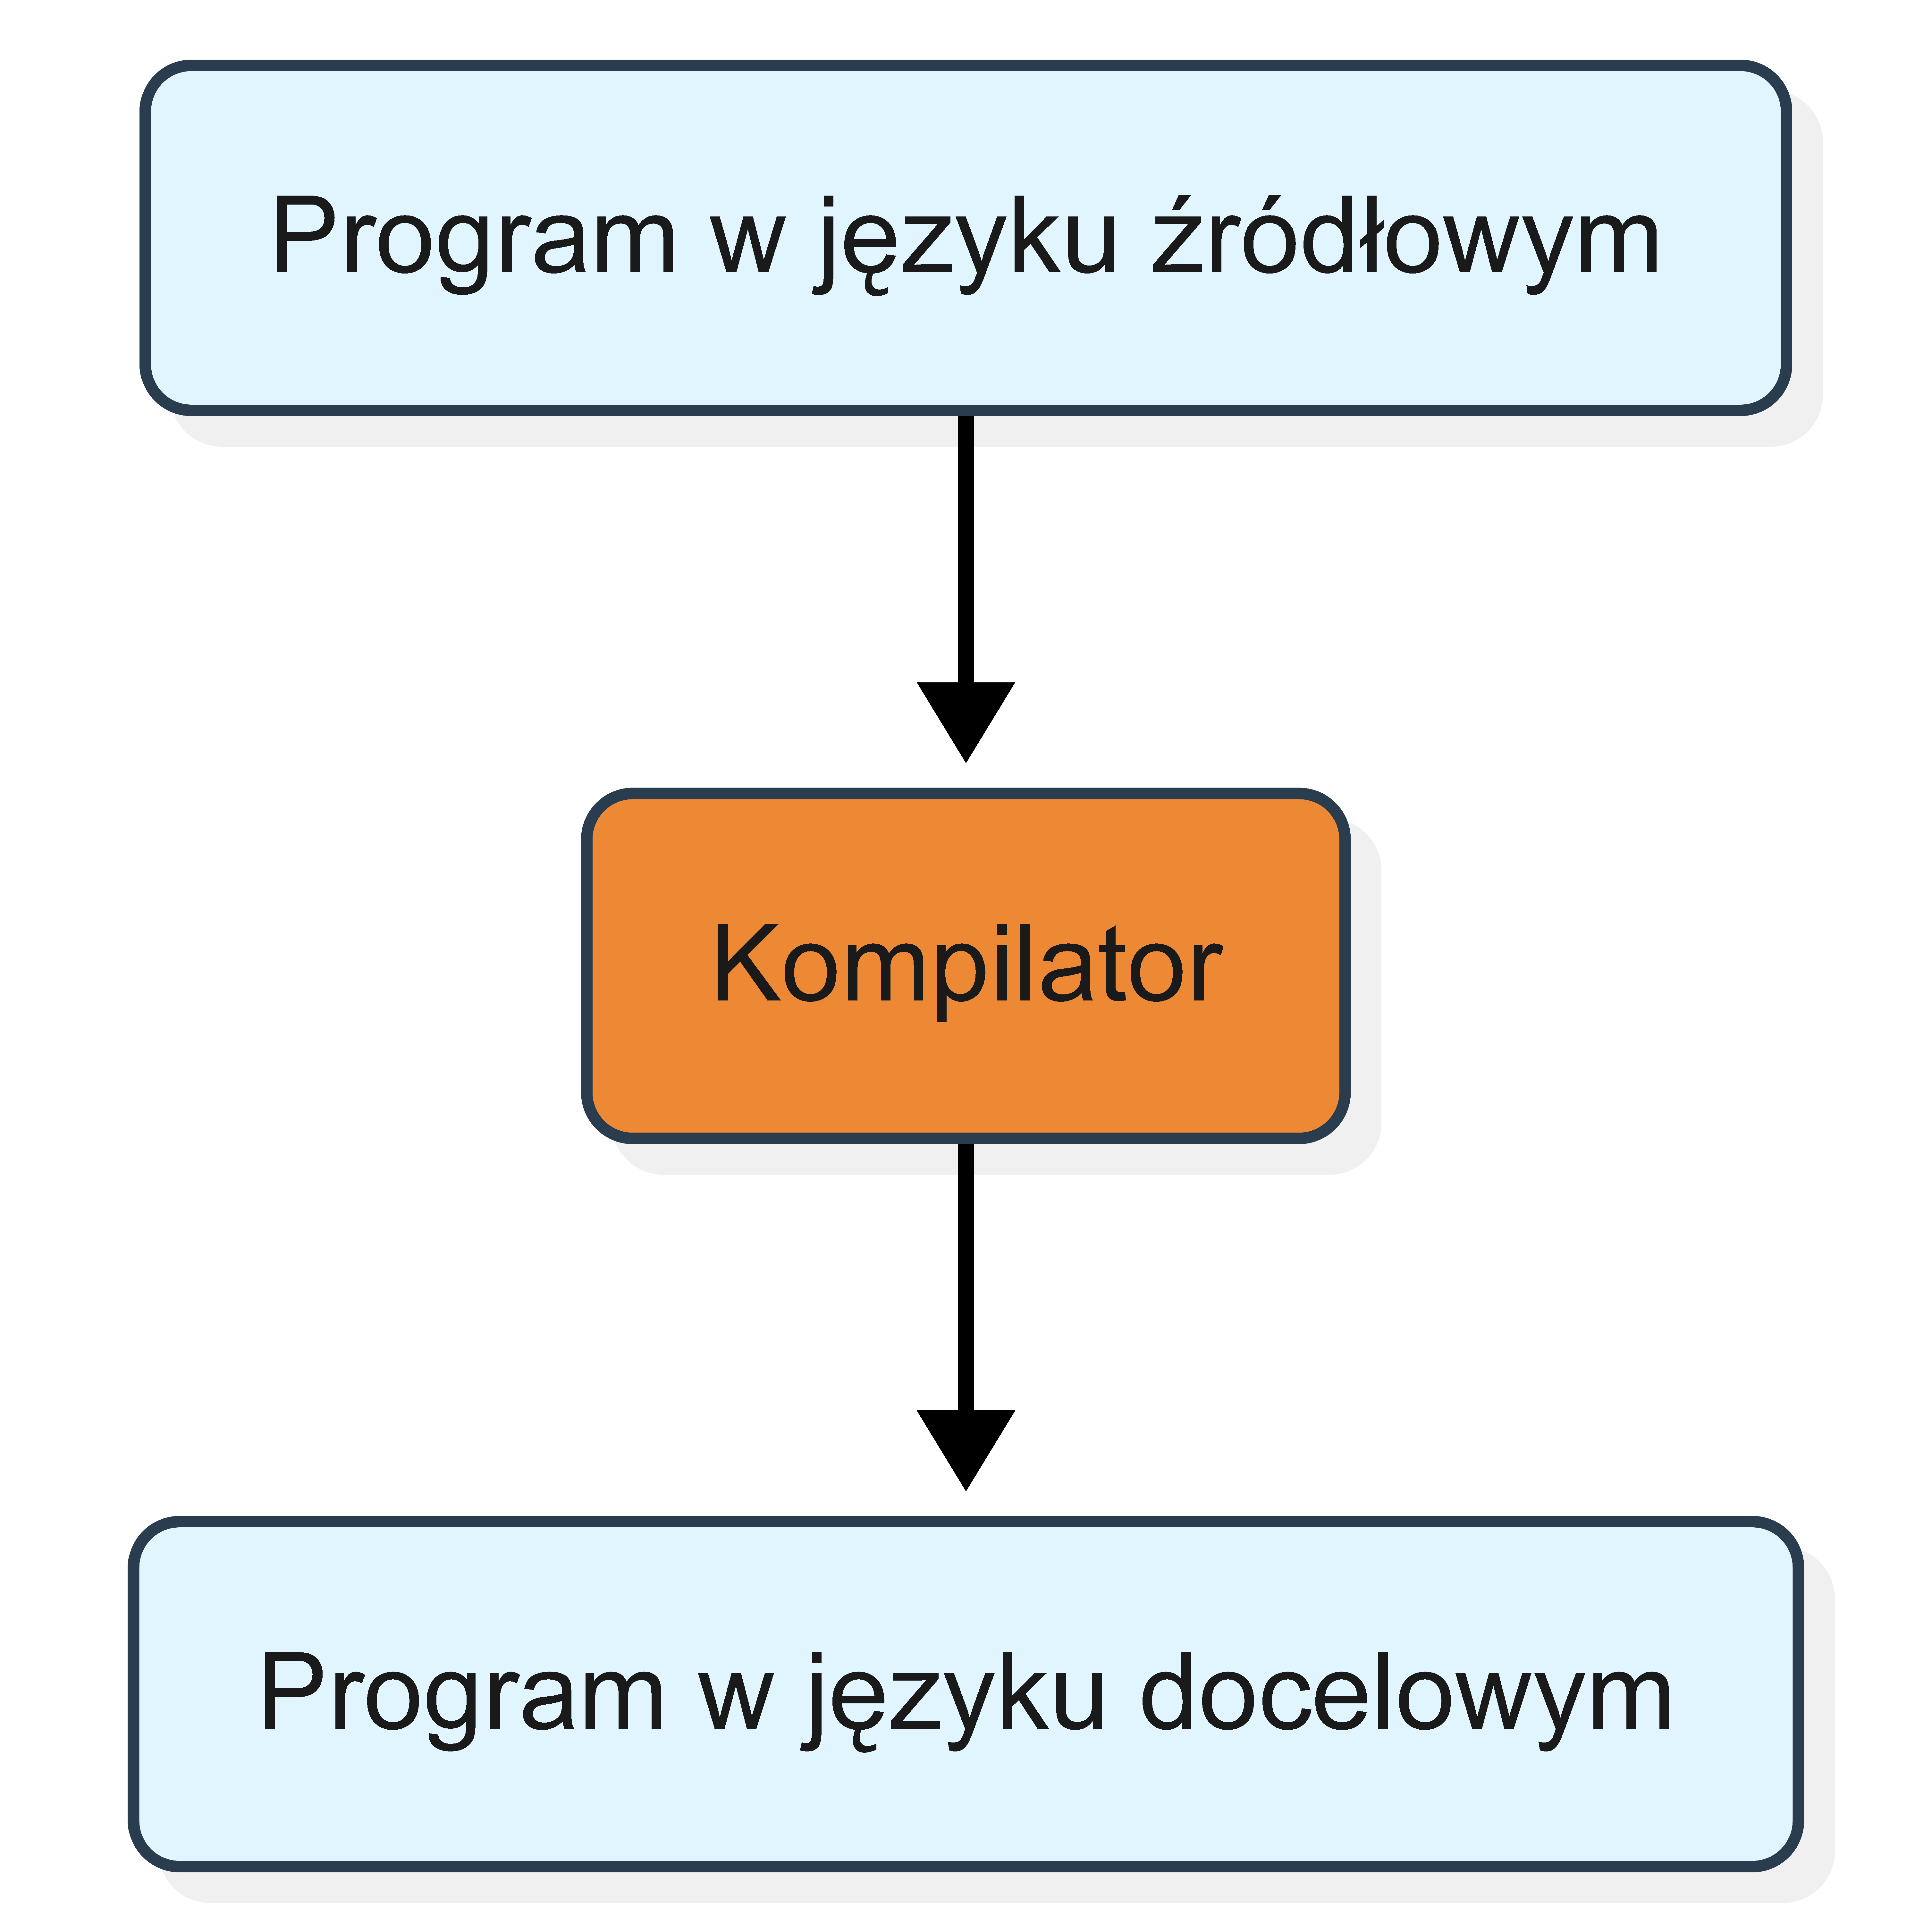
\includegraphics[width=0.6\textwidth]{img/Rysunek3.pdf}
    \caption{Model "czarnej skrzynki"~kompilatora}
    \label{fig:rysunek3}
\end{figure}

W systemach wbudowanych takie uproszczone podejście jest jednak często niewystarczające, ponieważ w takich zastosowaniach powszechnym zjawiskiem są silnie ograniczone zasoby sprzętowe, a nierzadko również ścisły rygor czasowy. Z tego względu programy tworzone przez inżyniera muszą być nie tylko poprawne pod kątem logicznym, ale również niezwykle rozsądnie gospodarować dostępnymi zasobami. Aby świadomie polepszać osiągi i kontrolować ten proces, konieczne jest porzucenie modelu czarnej skrzynki i zejście kilka poziomów abstrakcji niżej – począwszy od zrozumienia, jaki zestaw narzędzi jest w ogóle potrzebny do przetworzenia języka. 

Na potrzeby niniejszej pracy zostanie przytoczony sposób postępowania opisany w książce \cite{Kompilatory_Aho}, przedstawiony na schemacie \cref{fig:rysunek2}. Należy zaznaczyć, że zaprezentowany na rysunku pakiet oprogramowania, powszechnie określany jest przez użytkowników mianem kompilatora, choć w rzeczywistości zawiera w sobie zestaw wielu współpracujących programów komputerowych, w tym ten właściwy kompilator.
\begin{figure}[h]
    \centering
    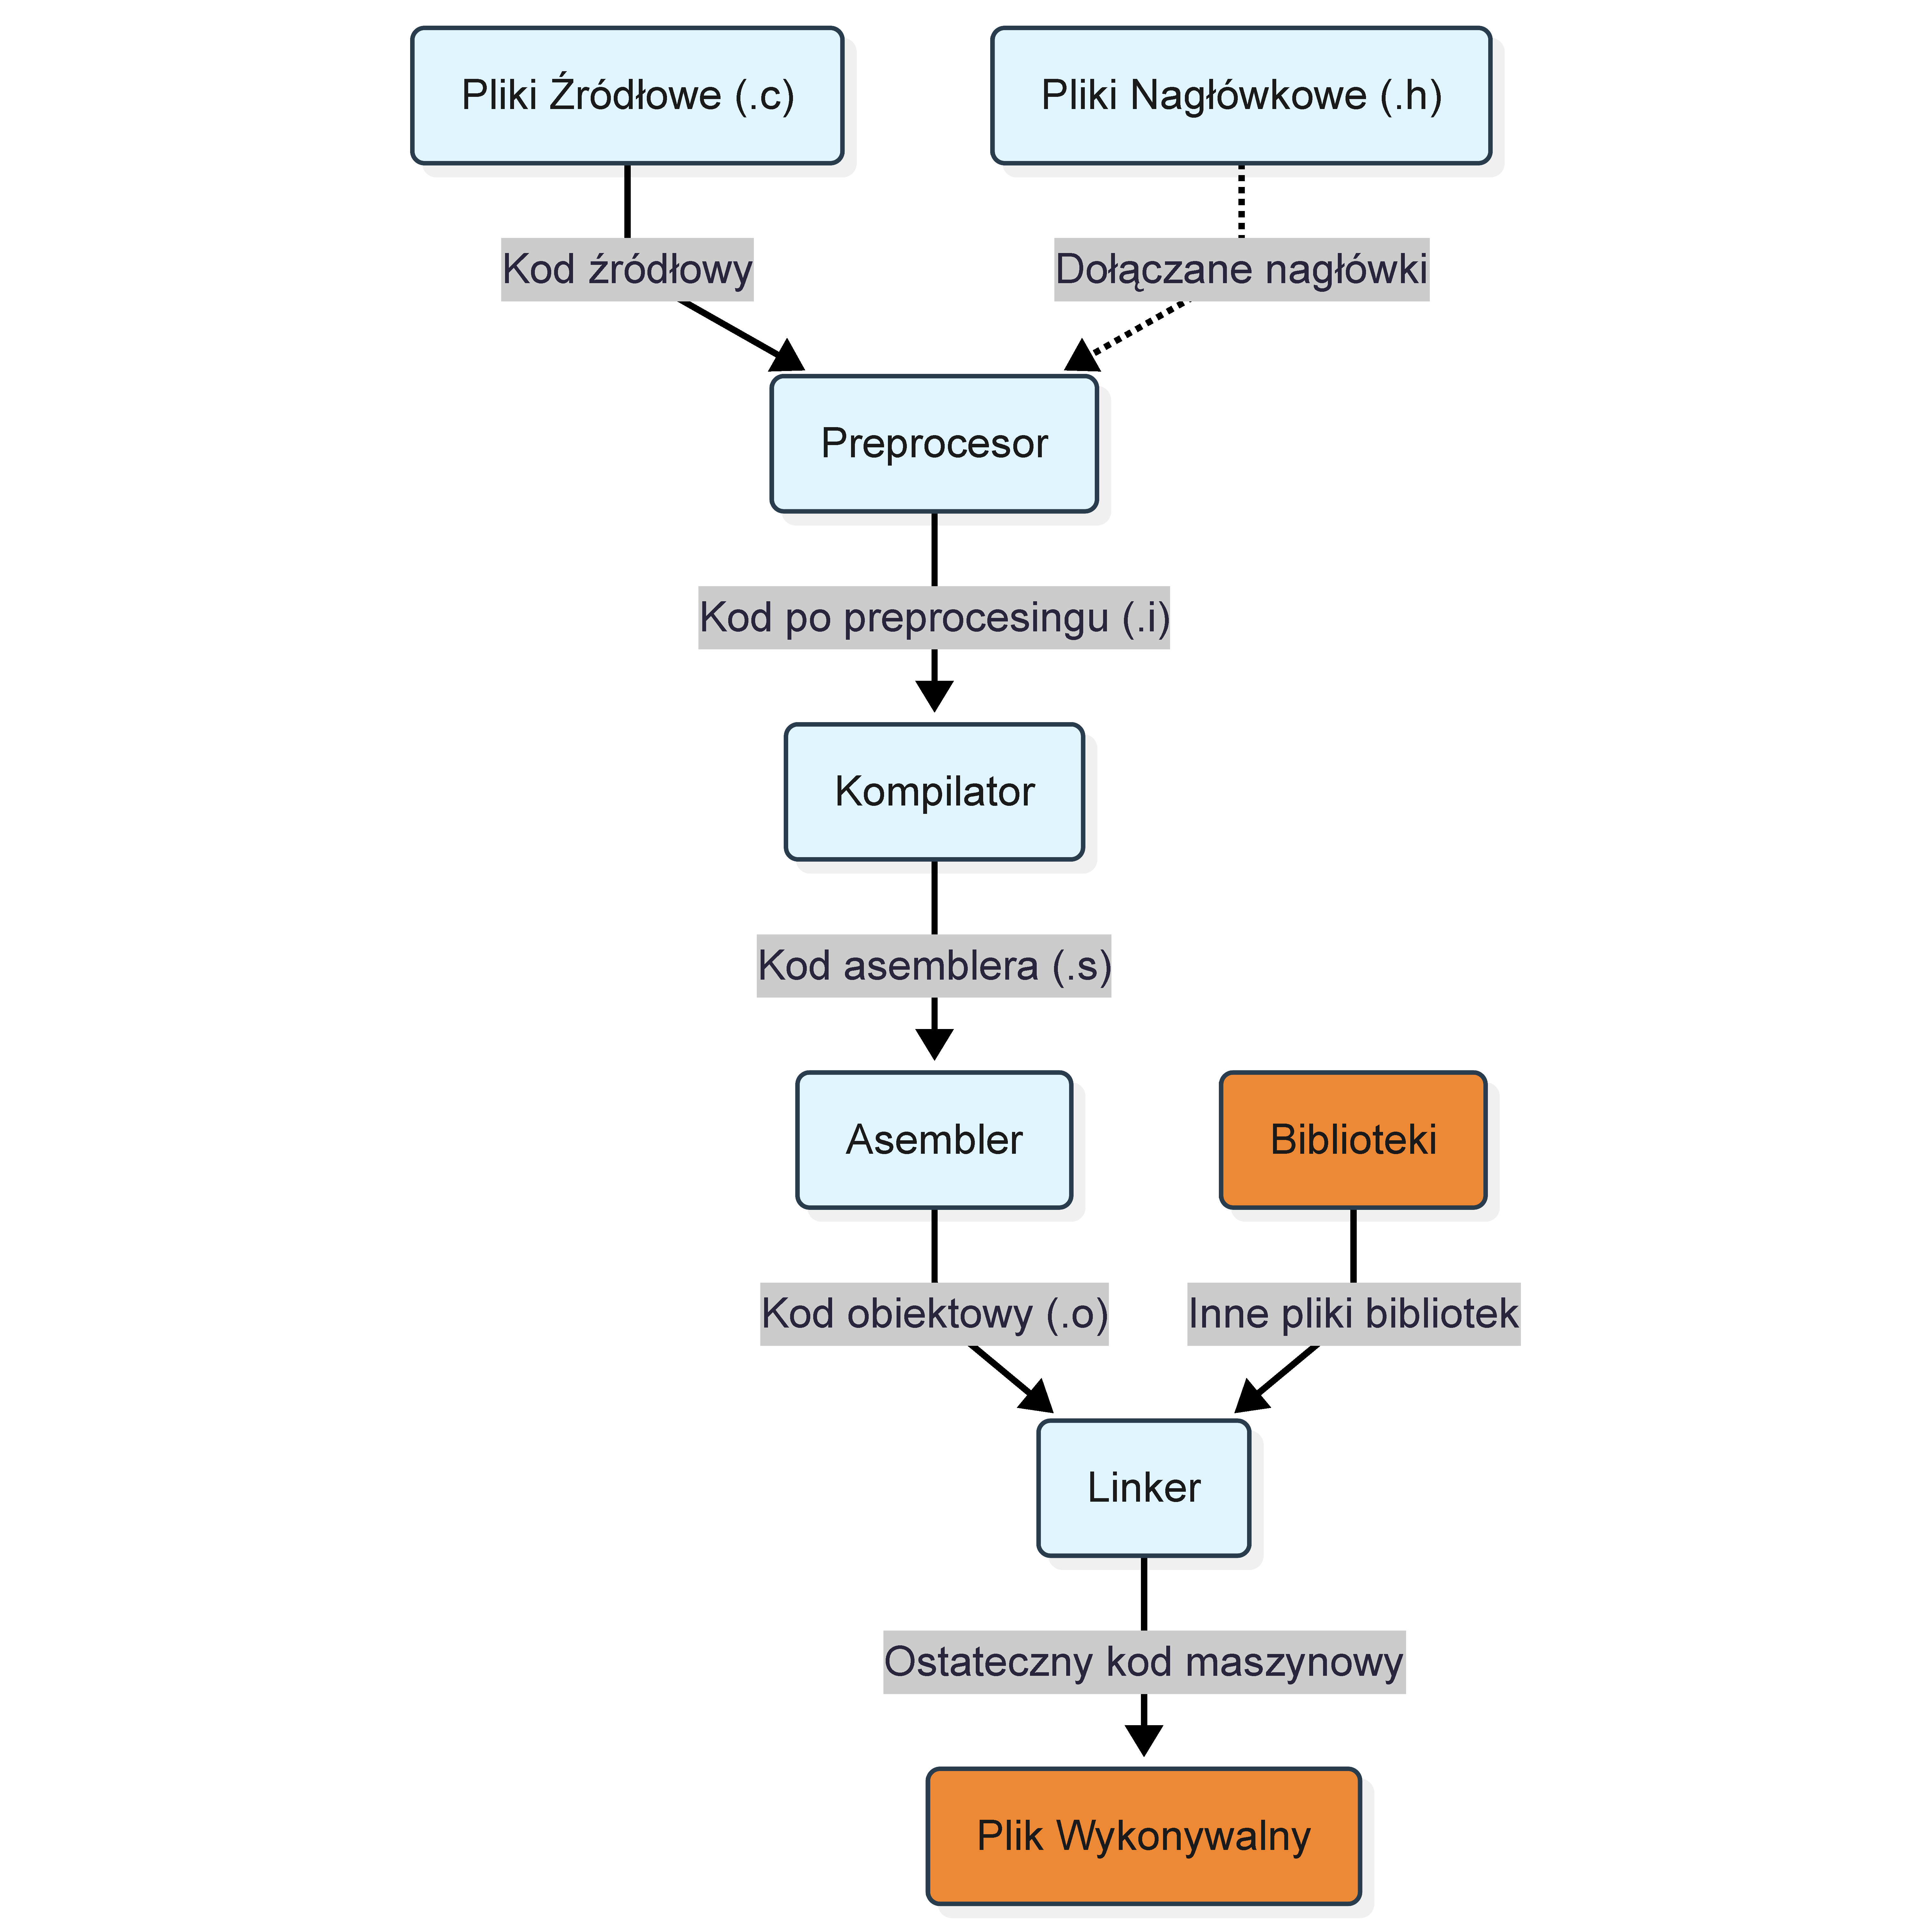
\includegraphics[width=0.8\textwidth]{img/Rysunek2.pdf}
    \caption{Klasyczny przebieg systemu przetwarzania języka programowania  \cite{Kompilatory_Aho}}
    \label{fig:rysunek2}
\end{figure}
Jak się okazuje, do utworzenia wykonywalnego programu docelowego wymagane jest najczęściej użycie kilku dodatkowych narzędzi, ułożonych w taki sposób, że wynik przetwarzania jednego jest wejściem dla kolejnego.
W klasycznym podejściu proces tworzenia pliku wykonywalnego składa się z następujących faz \cite{CinNutshell}:

\textbf{Preprocesor} odpowiada za przygotowanie kodu źródłowego przed jego właściwą analizą. Jego początkowym zadaniem jest zebranie programu, który nierzadko bywa podzielony na oddzielne moduły plikowe. Następnie program ten wykonuje odpowiednie dyrektywy oraz rozwija zdefiniowane przez programistę skróty (makra) do postaci pełnoprawnych instrukcji języka źródłowego.

\textbf{Kompilator} przyjmuje zmodyfikowany przez preprocesor kod i dokonuje jego tłumaczenia. Zazwyczaj wynikiem jego pracy nie jest bezpośredni kod maszynowy, lecz program zapisany w języku asemblera, powiązanym z docelową architekturą, na której uruchamiany ma zostać przygotowany program. Generowanie na tym etapie kodu asemblerowego wynika z faktu, iż jako język czytelny dla człowieka jest on znacznie łatwiejszy do wyprodukowania oraz ewentualnego debugowania.

\textbf{Asembler} zajmuje się przetworzeniem kodu asemblerowego na postać zrozumiałą dla maszyny. Wynikiem jego działania jest relokowalny kod maszynowy, zapisany w postaci tak zwanych plików obiektowych. Dodatkowo na tym etapie dla każdego z plików generowana jest tablica symboli, opisująca obiekty posiadające powiązania zewnętrzne \cite{CinNutshell}.

\textbf{Linker} łączy wygenerowane pliki obiektowe oraz niezbędne biblioteki w jeden spójny plik wykonywalny. Jego kluczowym zadaniem jest rozwiązanie adresów pamięci dla odwołań zewnętrznych pomiędzy poszczególnymi modułami programu, do czego wykorzystuje wspomniane wcześniej tablice symboli. W procesie tym linker dołącza również kod niezbędnych funkcji pochodzących ze standardowych lub zewnętrznych bibliotek \cite{CinNutshell}.

\subsection{Wewnętrzna struktura kompilatora}\label{subsection:WewStrukturaKompilatora}
%ta sekcja jest do poprawy, mamy 2 ksiazki compilter i dragon book z ktorych mozna sobie pokorzystac. 
Kompilator wewnętrznie dzieli się na dwie części: analizę (front end), która rozkłada program źródłowy na składowe elementy i na ich podstawie buduje reprezentację pośrednią oraz tablicę symboli, oraz syntezę (back end), która na tej podstawie konstruuje program docelowy \cite{Kompilatory_Aho}.

Proces ten przebiega jako sekwencja faz, z których każda przekształca jedną reprezentację programu w inną, a tablica symboli jest wykorzystywana przez wszystkie z nich \cite{Kompilatory_Aho}:

\begin{itemize}
    \item \textbf{Analiza leksykalna} - grupuje znaki programu źródłowego w leksemy i zamienia je na tokeny.
    \item \textbf{Analiza składniowa} - na podstawie tokenów buduje drzewo składniowe odzwierciedlające strukturę gramatyczną programu.
    \item \textbf{Analiza semantyczna} - sprawdza zgodność programu z definicją języka, w tym poprawność typów.
    \item \textbf{Generowanie kodu pośredniego} - tworzy niskopoziomową reprezentację programu, np. w postaci kodu trójadresowego.
    \item \textbf{Optymalizacja kodu} - opcjonalnie usprawnia kod pośredni, tak aby wynikowy kod docelowy był lepszy (np.\ szybszy lub mniejszy).
    \item \textbf{Generowanie kodu} - tłumaczy reprezentację pośrednią na kod maszyny docelowej, przydzielając m.in.\ rejestry zmiennym.
\end{itemize}

W praktycznych implementacjach kilka faz bywa łączonych w jeden przebieg (ang. \textit{pass}) \cite{Kompilatory_Aho}.


\section{Przegląd najpopularniejszych kompilatorów języka C}

Na rynku dostępnych jest wiele implementacji kompilatorów języka C, zarówno komercyjnych, jak i rozwijanych w modelu otwartoźródłowym. W praktyce jednak w środowisku systemów opartych na jądrze Linux najczęściej spotyka się dwa rozwiązania: \textbf{GNU Compiler Collection (GCC)}, powstały w ramach projektu GNU \cite{StallmanGNU}, oraz \textbf{Clang}, będący częścią projektu \textbf{LLVM}.\
Samo jądro systemu Linux przez długi okres było kompilowane było wyłącznie narzędziami GNU, jednak w ostanim czasie Clang i LLVM stały się dla nich dostepną alternatywą -- kompilowane z ich wykorzstaniem jądra systemu Linux wykorzystują między innymi systemy Android czy ChromeOS \cite{KernelLLVM}.

Warto zaznaczyć, że również w systemach wbudowanych, niewykorzystujących systemów operacyjnych, narzędzia GNU czy Clang wraz z LLVM są często spotykane. Oferują one wsparcie dla wielu architektur procesorów, pozwalając na uruchomienie kompilatora na sprzęcie o jednej architekturze (nazywanej również terminem \textbf{maszyny hosta}) w celu wygenerowania kodu maszynowego przeznaczonego dla zupełnie innej, docelowej architektury (nazywanej \textbf{maszyną targetu}). Proces ten określany jest mianem \textbf{kompilacji skrośnej} (ang. \textit{cross-compilation}). Obydwa wspomniane kompilatory posiadają zestaw narzędzi przeznaczonych do różnych architektur spotykanych w systemach wbudowanych, takich jak \textbf{ARM, RISC-V, AVR}.
\subsection{Kompilator GCC}

\textbf{GCC} powstał jako część projektu GNU \cite{StallmanGNU} i jest tradycyjnym, domyślnym kompilatorem większości dystrybucji systemu Linux \cite{LinuxKernelDevelopment}. Jego architektura rozwiązań bazuje na klasycznym modelu kompilatora, który opisuje \cref{subsection:WewStrukturaKompilatora}. GCC dzieli proces tłumaczenia na część analizującą (front end) i część generującą kod wynikowy (back end). Część środkowa, odpowiedzialna za optymalizacje, przekształca program w dwóch własnych, uproszczonych reprezentacjach -- GENERIC oraz GIMPLE -- na których wykonywane są kolejne przekształcenia mające na celu poprawnienie kodu \cite{novillo2006gcc}. 
\subsection{Kompilator Clang}

\textbf{Clang} pełni rolę części analizującej (front end) dla  części syntezy obsługiwanej przez \textbf{LLVM}. LLVM zapewnia zestawu narzędzi kompilatorowych, zaprojektowanego tak, aby umożliwić analizę i poprawianie kodu na każdym etapie jego translacji i uruchomienia \cite{lattner2004llvm}. Podobnie jak GCC, LLVM przekształca program do własnej, uproszczonej reprezentacji pośredniej, jednak w odróżnieniu od GCC reprezentacja ta została zaprojektowana w taki sposób, aby nie musięć zależeć od konkretnego języka programowania \cite{lattner2004llvm}. Dzięki takiej budowie LLVM można podzielić na trzy niezależne części: część analizującą (Clang), wspólną dla wszystkich architektur warstwę optymalizacji oraz część generującą kod maszynowy dla konkretnego procesora. Kod projektu LLVM, w tym Clang, jest udostępniany na licencji Apache License \cite{LLVMDevPolicy}.

Oba kompilatory, mimo różnic w budowie wewnętrznej, są ze sobą często porównywane w literaturze pod kątem jakości i wydajności generowanego kodu, w tym w zastosowaniach wbudowanych systemów wbudowanych \cite{poorhosseini2020compiler}.Oba rozwiązania dysponują bowiem wbudowanymi mechanizmami zaawansowanej optymalizacji kodu, o których traktuje \cref{section:TechnikiOptymalizacji}. Proces ten może być kontrolowany przez inżyniera oprogramowania poprzez stosowanie \textbf{flag kompilacji}, czyli poleceń określających pożądany stopień i cel optymalizacji programu docelowego. \cref{section:flagiKompilatora} przybliża dostępne flagi dla obywdu opisywanych kompilatorów.
\section{Zaawansowane techniki optymalizacji kodu}\label{section:TechnikiOptymalizacji}
\section{Flagi kompilacji dostępne w kompilatorach Clang i Gcc}\label{section:flagiKompilatora}

\begin{table}[htbp]
    \centering
    \caption{Poziomy optymalizacji w kompilatorach GCC i Clang, na podstawie oficjalnych dokumentacji\cite{gcc_optlevels,clang_cmdguide}}
    \label{tab:poziomy_optymalizacji}
    \begin{tabularx}{\textwidth}{@{} l X X @{}}
        \toprule
        \textbf{Flaga} & \textbf{GCC} & \textbf{Clang} \\
        \midrule

        \texttt{-O0} &
            Brak optymalizacji (ustawienie domyślne). Generuje nieoptymalny kod, lecz zapewnia najkrótszy czas kompilacji i najlepsze warunki do debugowania. &
            Oznacza brak optymalizacji -- najszybsza kompilacja i najlepiej debugowalny kod wynikowy. \\
        \addlinespace

        \texttt{-O1} &
            Umiarkowana optymalizacja (odpowiednik samego \texttt{-O}). Rozsądnie optymalizuje kod bez istotnego wydłużenia czasu kompilacji, choć część zmiennych może być niedostępna w debuggerze. &
            Poziom pośredni między \texttt{-O0} a \texttt{-O2}. \\
        \addlinespace

        \texttt{-O2} &
            Rozszerzona optymalizacja generująca silnie zoptymalizowany kod kosztem wydłużonego czasu kompilacji; istotnie utrudnia pracę z debuggerem. &
            Umiarkowany poziom optymalizacji włączający większość dostępnych optymalizacji. \\
        \addlinespace

        \texttt{-O3} &
            Pełna optymalizacja obejmująca bardziej zaawansowane przekształcenia, zwłaszcza pętli, potencjalnie kosztem większego rozmiaru kodu wynikowego. Praca z debuggerem jest w praktyce bardzo utrudniona. &
            Odpowiednik \texttt{-O2} rozszerzony o optymalizacje wymagające dłuższego czasu kompilacji lub zwiększające rozmiar kodu, w celu poprawy szybkości wykonania. \\
        \addlinespace

        \texttt{-Os} &
            Optymalizacja pod kątem rozmiaru kodu i danych zamiast szybkości; bazuje na \texttt{-O2} z wyłączeniem przekształceń zwiększających rozmiar binarki oraz dodatkowymi optymalizacjami redukującymi rozmiar. &
            Odpowiednik \texttt{-O2} z dodatkowymi optymalizacjami zmniejszającymi rozmiar kodu wynikowego. \\
        \addlinespace

        \texttt{-Oz} &
            Agresywna optymalizacja rozmiaru kodu i danych; może zwiększyć liczbę wykonywanych instrukcji, jeśli wymagają one mniejszej liczby bajtów do zakodowania. &
            Odpowiednik \texttt{-Os}, lecz z jeszcze dalszą redukcją rozmiaru kodu wynikowego. \\
        \addlinespace

        \texttt{-Og} &
            Optymalizacja zorientowana na komfort debugowania zamiast szybkości; bazuje na \texttt{-O1}, dążąc do wyeliminowania negatywnego wpływu optymalizacji na proces debugowania. &
            Zbliżony do \texttt{-O1}, lecz z nieco ograniczoną optymalizacją i lepszą widocznością zmiennych; dodatkowo ustawia flagę \texttt{-fextend-variable-liveness}, poprawiającą dostępność zmiennych podczas debugowania. \\
        \addlinespace

        \texttt{-Ofast} &
            Poziom nieuwzględniony w cytowanym dokumencie GNAT jako osobna flaga GCC (w praktyce GCC obsługuje \texttt{-Ofast} analogicznie do Clang -- zob.\ kolumna obok). &
            Włącza wszystkie optymalizacje z \texttt{-O3} wraz z dodatkowymi agresywnymi optymalizacjami mogącymi naruszać ścisłą zgodność ze standardem języka (m.in.\ \texttt{-ffast-math}). Flaga oznaczona jako przestarzała od Clang 19. \\

        \bottomrule
    \end{tabularx}

    \vspace{0.5em}
\end{table}




\chapter{Projekt systemu testowego i metodyka przeprowadzonych badań}\label{}
%Tutaj trzeba kilka razy do znudzenia powtorzyc o naszym celu badan

\section{Zaimplementowane warianty algorytmu FFT}\label{section:WariantyFFTUzyteWPracy}
%tutaj piszemy krotko o kazdym algorytmie uzytym i uzasadniamy dlaczego on jest wybrany do badan
\section{Opis plattformy sprzetowej}\label{}
%Nie za dlugi, moze jakis obrazek z creativecommons, ale nie wiem jak go sie cytuje
\subsection{Jednostka Neon}\label{subsection:jednostkaNeon}
\section{Założenia projektowe i architektura aplikacji}
\subsection{Weryfikacja poprawności obliczeń z biblioteka zewnetrzna}
\section{Użyte biblioteki i narzędzia programistyczne}
%Tutaj trzeba napisac co optymalizujemy, w jaki sposob i jakie sa z tym problemy    

%Tu trzeba napisac o pomiarach czasu, bibliotekach do patrzenia na to, cross kompilacji, sprawdzaniu uzyciu stosu, wykorzystania stosu, etc
% Mozna cos wspominiec o deasemblacji i porownywaniu kodow asemblera

\section{Metodyka przeprowadzonych pomiarów}

\chapter{Przeprowadzone badania}\label{WykonaneBadania}
Głównym celem niniejszej pracy były badania wpływu wybranych funkcji sąsiedztwa na możliwość późniejszego wykorzystania sieci samoorganizujących w zadaniach klasyfikacji danych. Do przeprowadzenia badań wykorzystano implementację opisaną w rozdziale \ref{Opis_rozwiazania}. 
\\Badania przeprowadzono na trzech popularnych zbiorach uczących: "MNIST" \cite{MNIST}, "IRIS" \cite{IRIS} i \\Cardiotocography\cite{Patologie}. Każdy z tych zbiorów danych zostanie szczegółowo opisany w osobnej sekcji prezentowanego rozdziału.

W badaniach skupiono się na analizie wpływu wybranej funkcji sąsiedztwa na wartość błędu kwantyzacji, błędu topograficznego i na ocenie jakości klasteryzacji danych na podstawie uzyskanych map zwycięzców. Porównano również dwie rozbieżne kwestie podnoszone w literaturze – dotyczące natury promienia w sieciach SOM. Rozważano, czy promienie sąsiedztwa powinny przyjmować wyłącznie wartości całkowite, tak jak opisano to w pozycji \cite{Kohonen}, czy też mogą być liczbami niecałkowitymi, tak jak przedstawiono to w \cite{Haykin}. Porównania dokonano dla dwóch topologii sieci - prostokątnej z ośmioma sąsiadami i heksagonalnej. 

W celu realizacji postawionych założeń przyjęto jednolitą metodologię badań, opisaną w sekcji \ref{metodologiaBadań}.

\section{Metodologia badań}\label{metodologiaBadań}

Procedura wykonywania badań była jednakowa dla każdego zbioru uczącego. Początkowym etapem było wczytanie danych do programu i wstępne ich przetworzenie. Na tym etapie zbiór danych dzielony był na zbiór uczący i zbiór testowy, w proporcjach osiemdziesiąt (80) do dwudziestu (20) procent. Wyjątkiem tutaj były badanie na zbiorze IRIS, co uzasadniono w sekcji \ref{Irys_sekcja}. Następnie wszystkie dane były normalizowane, do zakresu od zera do jeden. Normalizacja przebiegała według wzoru \ref{normalizacja}.
\begin{equation} \label{normalizacja}
z' = a_g + \frac{(z - z_{\text{min}})}{(z_{\text{max}} - z_{\text{min}})} \cdot (b_g - a_g),
\end{equation}
gdzie \( z \) oznacza oryginalną wartość w zbiorze danych, \( z' \) to przeskalowana wartość, \( z_{\text{min}} \) i \( z_{\text{max}} \) reprezentują odpowiednio minimalną i maksymalną wartość w kolumnie danych, zaś \( a_g \) i \( b_g \) to granice przedziału skalowania ( \( a_g = 0 \) oraz \( b_g = 1 \)).

Liczba epok oraz parametry sieci były dostosowywane indywidualnie dla każdego zbioru uczącego, zgodnie z zasadami zaprezentowanymi w sekcji \ref{Zasady_doboru_parametrow}. Wartości tych parametrów pozostawały takie same dla wszystkich funkcji sąsiedztwa użytych przy treningu i ewaluacji modeli. Również funkcje zmiany współczynnika uczenia i zasięgu sąsiedztwa były jednolite w obrębie każdego zbioru uczącego. Pewną stałą wśród wszystkich badań była zastosowana miara odległości między wzorcami wejściowymi, a wektorami wag. Użyto miary euklidesowej, opisanej w sekcji \ref{eq:euklidesowa}, ze względu na jej popularność w innych pracach \cite{Kohonen,breast,Marine_Traffic}.

Ewaluacja modeli polegała na wyznaczeniu wartości średniego błędu kwantyzacji oraz błędu topograficznego, na danych testowych, dla każdego modelu, stworzonego z zastosowaniem innej funkcji sąsiedztwa w procesie uczenia. Tworzone były również mapy zwycięzców do wizualnej oceny jakości klasteryzacji.

W kolejnych sekcjach rozdziału zaprezentowano osiągnięte rezultaty. W każdej z sekcji \ref{Irys_sekcja}, \ref{Patologie_sekcja} oraz \ref{MNIST_sekcja} opisano wykorzystany zbiór uczący wraz z uzasadnieniem wyboru. Umieszczono w nich także tabele z porównaniem wartości średnich błędów kwantyzacji i topograficznego oraz mapę zwycięzców dla modelu z najmniejszym wynikami obu błędów. Zdecydowano się na prezentację tylko jednej z map zwycięzców, z uwagi na ilość wytrenowanych modeli.

%IRYSY SEKCJA

\section{Badania na zbiorze IRIS}\label{Irys_sekcja}
Zbiór danych \textit{Iris} jest jednym z najpopularniejszych zbiorów danych wykorzystywanych w zadaniach klasyfikacji i klasteryzacji. Przez swoją prostą strukturę, umożliwia wstępne zbadanie wszelkiego rodzaju algorytmów analizy danych, dlatego jest częstym przedmiotem badań \cite{IRIS}. Zbiór ten powstał w 1936 roku i zawiera 150 próbek opisujących 3 gatunki  irysów (roślina ozdobna). Każdy wektor danych zawiera cztery cechy opisujące morfologię kwiatu tej rośliny: długość działki kielicha (\textit{sepal length}), szerokość działki kielicha (\textit{sepal width}), długość płatka (\textit{petal length}) oraz szerokość płatka (\textit{petal width}).
\\Dane wejściowe podzielone są na 3 klasy, reprezentujące różne gatunki rośliny:
\begin{itemize}
\item \textbf{Setosa}:  50 próbek, z etykietą "0",
\item \textbf{Versicolor}:  50 próbek, z etykietą "1"
\item \textbf{Virginica}:  50 próbek, z etykietą "2".
\end{itemize}

Zbiór danych wydaje się z pozoru prosty do klasyfikacji, ze względu na swoją wielkość i ograniczoną liczbę cech. Problemy może jednak sprawiać specyficzny podział na klasy, występujący w tym zbiorze. Wynika to z faktu, że irysy z gatunku \textbf{Versicolor} mają podobną budowę morfologiczną, jak irysy z gatunku \textbf{Virginica}. 
Prowadzi to często do trudności w jednoznacznej klasyfikacji tych roślin.

Zbiór danych został wybrany z uwagi na niewielki rozmiar, równą liczność klas oraz ograniczoną liczbę cech. W badaniu skupiono się na ocenie działania sieci samoorganizującej się w takim zbiorze, a także na analizie jej zdolności do zachowania topologii danych. Zakłada się, że taka właściwość sieci SOM powinna prowadzić do wyraźnego oddzielenia danych należących do klasy \textit{Setosa} od pozostałych, natomiast dane z klas \textit{Versicolor} i \textit{Virginica}, ze względu na ich podobieństwo, mogą częściowo się nakładać na mapie zwycięzców.

Do tworzenia modeli wykorzystano siatkę 8 na 8 neuronów, z początkowym promieniem równym 4 i początkową wartością współczynnika uczenia równą 0.3. Wykorzystano funkcję liniową, opisaną w sekcji \ref{eq:linear_decay}, dla zmiany wartości promienia  oraz funkcję wymierną, opisaną w sekcji \ref{eq:exponential_decay},  dla zmiany wartości współczynnika uczenia. Ze względu na ograniczoną liczbę danych w zbiorze, każda z sieci była trenowane przez 10000 epok.

W przypadku tego (dość małego zbioru) zbioru, dane nie były dzielone na zbiór uczący i testowy. Skutkowało to ewaluacją modeli na tych samych danych, na których przeprowadzone zostało uczenie sieci. Sieć Kohonena potraktowano tutaj jako narzędzie do analizy i klasyfikacji danych wyłącznie w obrębie zbioru uczącego. Takie zastosowanie sieci jest również popularne, między innymi w pozycji \cite{breast}.

Tabela \ref{IRIS_tabela} przedstawia otrzymane wartości błędów kwantyzacji i topograficznych. Zastosowane skróty oznaczają kolejno: \(\textbf{hex}_{ncp}\) – badania dla topologii heksagonalnej i niecałkowitych wartości promienia, \(\textbf{rect}_{ncp}\) – badania dla topologii prostokątnej z ośmioma sąsiadami i niecałkowitych wartości promienia, \(\textbf{hex}_{cp}\) – badania dla topologii heksagonalnej i całkowitych wartości promienia, oraz \(\textbf{rect}_{cp}\) – badania dla topologii prostokątnej z ośmioma sąsiadami i całkowitych wartości promienia.
\begin{table}[h]
\centering
\caption{Wartości błędów topograficznych i kwantyzacji  z testów na zbiorze IRIS}
\label{IRIS_tabela}
\begin{tabular}{|l|l|l|l|l|l|}
\hline
\textbf{\begin{tabular}[c]{@{}l@{}}funkcja\\ sasiedztwa\end{tabular}} & \textbf{Rodzaj błędu} & \(\textbf{hex}_{ncp}\) & \(\textbf{rect}_{ncp}\) & \(\textbf{hex}_{cp}\) & \(\textbf{rect}_{cp}\) \\ \hline
\multirow{2}{*}{\textbf{Gaussa}}                                      & błąd kwantyzacji      & 0.0837                 & 0.0946                  & 0.0931                & 0.0936                 \\ \cline{2-2}
                                                                      & błąd topograficzny    & 0.0063                & 0.1128                  & 0.0338                & 0.0902                 \\ \hline
\multirow{2}{*}{\textbf{trójkątna}}                                   & błąd kwantyzacji      & 0.0630                 & 0.0626                  & 0.0574                & 0.0576                 \\ \cline{2-2}
                                                                      & błąd topograficzny    & 0.0812                 & 0.2066                  & 0.1123                & 0.2130                 \\ \hline
\multirow{2}{*}{\textbf{prostokątna}}                                     & błąd kwantyzacji      & 0.0942                 & 0.0805                  & 0.0858                & 0.0769                 \\ \cline{2-2}
                                                                      & błąd topograficzny    & 0.0096                 & 0.1153                  & 0.0420                & 0.1430                 \\ \hline
\multirow{2}{*}{\textbf{eksponencjalna}}                              & błąd kwantyzacji      & 0.0810                 & 0.0769                  & 0.0820                & 0.0741                 \\ \cline{2-2}
                                                                      & błąd topograficzny    & 0.0600                 & 0.1133                  & 0.0661                & 0.1532                 \\ \hline
\end{tabular}
\end{table}

\subsection{Wnioski z badań na zbiorze IRIS}
Maksymalny błąd kwantyzacji dla tego zbioru danych, zdefiniowany zależnością \ref{maksymalny_blad_kwantyzacji} przyjmuje wartość\(\sqrt{4} =2\). Najlepszą z uzyskanych wartości w przypadku tego błędu, wynosi 0.0574 i stanowi \(2.87\%\) wartości maksymalnej. Otrzymano ją  dla zastosowania funkcji trójkątnej, z promieniem sąsiedztwa zmieniającym się w sposób całkowity oraz topologią heksagonalną. W tym wypadku wystąpił jednak  znaczny błąd topograficzny, co przeniosło się bezpośrednio na rozkład klas na mapie zwycięzców. Podobnie, przy innych sieciach trenowanych za pomocą tej funkcji osiągnięto wysokie błędy topograficzne, które uniemożliwiają skuteczne stosowanie zaproponowanej funkcji trójkątnej w tym przypadku. Otrzymane rezultaty mogą wynikać z postaci funkcji trójkątnej stosowanej w zaproponowanej implementacji.
Szersze skomentowanie wyników błędów otrzymanych przy trenowaniu sieci z użyciem funkcji trójkątnej przedstawiono w rozdziale \ref{Podsumowanie_badań}.

Użycie funkcji eksponencjalnej pozwoliło na zmniejszenie wartości błędów topograficznych, w stosunku do ich wartości w przypadku stosowania funkcji trójkątnej. 
Zadowalające rezultaty osiągnięto także przy zastosowaniu funkcji progowej. W każdej możliwej kombinacji topologia - sposób zmiany promienia, osiągnięto rezultaty nieznacznie gorsze od funkcji Gaussa. Jest to dość nieoczekiwana obserwacja, która może sugerować, że dla prostych zbiorów danych stosowanie funkcji progowej jest warte rozważenia.

Najmniejsze wartości błędu kwantyzacji i topograficznego, wraz z najlepszymi rezultatami na mapie zwycięzców, osiągnięto przy stosowaniu funkcji Gaussa w topologii heksagonalnej wraz ze zmniejszającym się w sposób niecałkowity promieniem. Wynik takiego grupowania przedstawiono na rysunku \ref{fig:Iris_best}. Przy zastosowaniu topologii prostokątnej również osiągano zadowalające wartości błędów, w zestawieniu z innymi funkcji sąsiedztwa. Zmiana sposobu określania promienia na całkowity spowodowała zwiększenie błędów topograficznych, tym samym pogarszając jakość grupowania na mapie zwycięzców.

Grupowanie klas zaprezentowane na rysunku \ref{fig:Iris_best} spełnia oczekiwania, wskazując na widoczne klastry odpowiadające poszczególnym etykietom danych. Szczególnie zauważalna jest strefa bez zwycięzców, między danymi z etykietą 0 a 1, co jest zgodne z teoretycznymi założeniami dotyczącymi zdolności sieci SOM do zachowywania relacji w danych. Takie rozmieszczenie odzwierciedla naturalne odseparowanie tych dwóch analizowanych gatunków irysów, wspomniane na wstępie tej sekcji. Z kolei dane z etykietami 1 i 2 reprezentowane są przez neurony położone blisko siebie, aż do przypadków nachodzenia na siebie. Prezentowana mapa zwycięzców  wiernie odwzorowuje  rzeczywisty układ danych w zbiorze IRIS.
\\Osiągnięte rezultaty wskazują, że istnieje możliwość skutecznego wykorzystania sieci SOM do klasyfikacji danych o niewielkiej liczbie wymiarów i zrównoważonej liczności elementów w poszczególnych klasach, przy jednoczesnym zachowaniu ich zależności topologicznych, tak jak  zostało to  zaobserwowane przy analizie badań na zbiorze Iris.  
\begin{figure}[h]
    \centering
    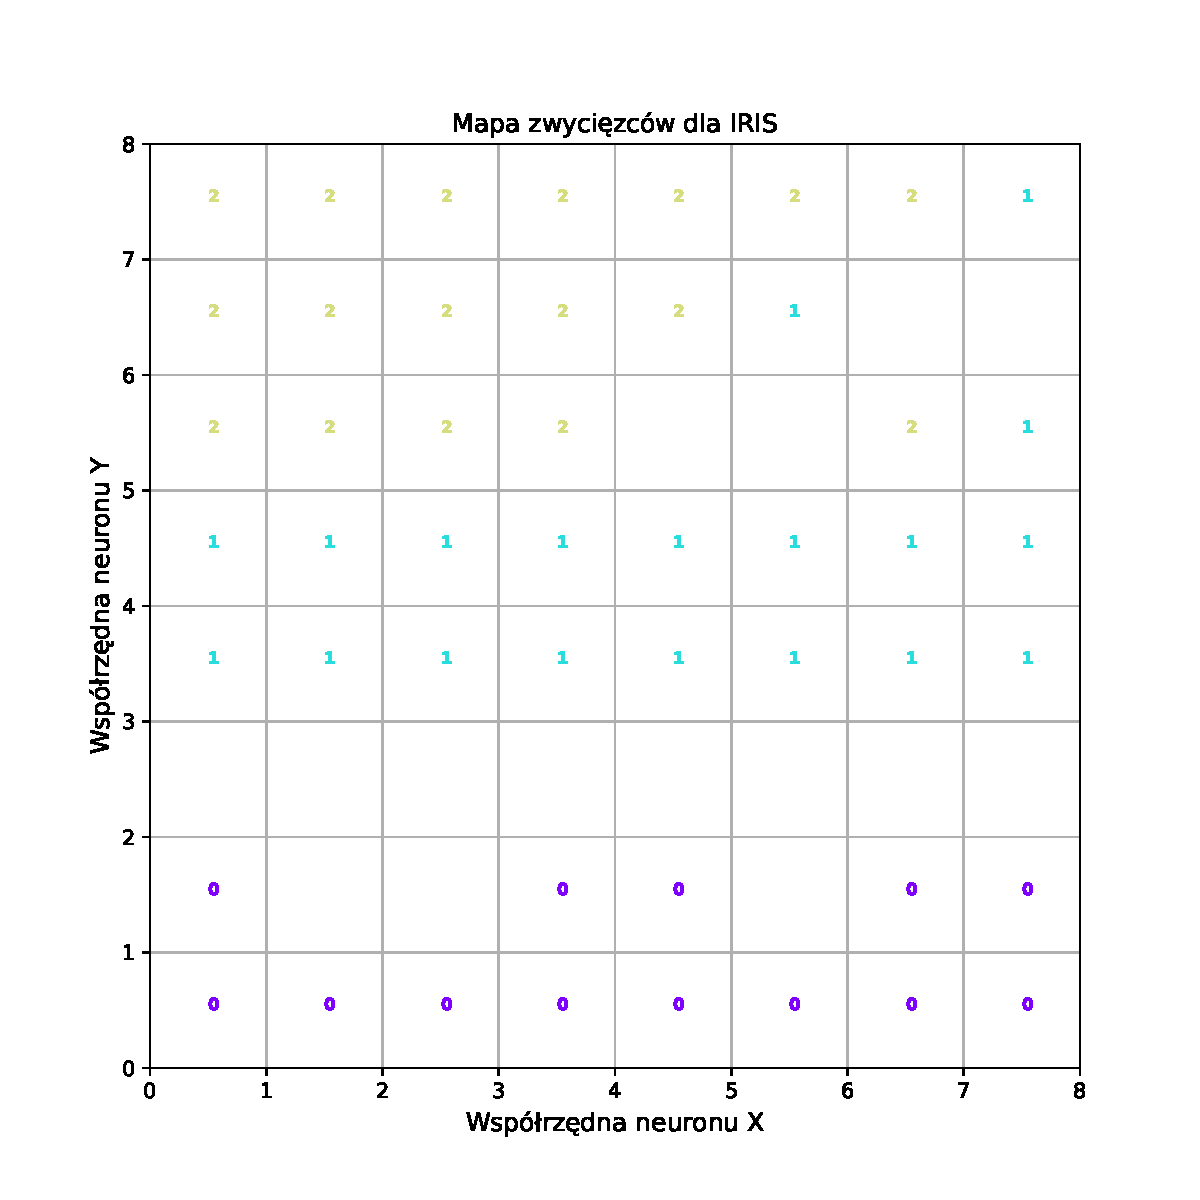
\includegraphics[width=0.8\textwidth]{./img/Iris_best.pdf}
    \caption{Mapa zwycięzców otrzymana w wyniku testów na zbiorze  IRIS}
    \label{fig:Iris_best}
\end{figure}

%PATOLOGIE SEKCJA
\section{Badania na zbiorze Cardiotocography}\label{Patologie_sekcja}
Zbiór danych Cardiotocography zawiera dane medyczne pozyskane z badań kardiotokografi (CTG), analizujących akcję serca płodu ludzkiego. Informacje umieszczone w tym zbiorze zostały udostępnione przez Instytut Położnictwa i Ginekologii Uniwersytetu Medycznego w Porto w Portugalii \cite{Patologie}. Zbiór danych zawiera 2126 próbek, każda z 21 cechami, takimi jak liczba uderzeń serca na minutę, czy liczba ruchów płodu. Oprócz cech każda z wartości ma przypisaną jedną z trzech etykiet, przypisanych przez lekarzy położników:
\begin{itemize}
    \item 1 - \textbf{Normalny (ang. Normal)}: oznaczający brak problemów zdrowotnych, liczność podzbioru danych wynosi 1655,
    \item 2 - \textbf{Podejrzany (ang. Suspect)}: wymagający dalszej obserwacji, liczność podzbioru danych wynosi 295,
    \item 3 - \textbf{Patologiczny (ang. Pathologic)}: wskazujący na możliwe komplikacje, liczność podzbioru danych wynosi 176.
\end{itemize}

Z punktu widzenia analizy danych zbiór uczący zawiera niewiele klas, za to dane posiadają wiele wymiarów. Należy również uwzględnić, że jedna z tych klas jest zdecydowanie dominująca. Wyboru dokonano zarówno ze względu na praktyczną możliwość wykorzystania sieci SOM jako narzędzia wspomagającego pracę w tak istotnej dziedzinie jak medycyna, jak i przez czysto techniczną potrzebę zbadania możliwości wykorzystania sieci przy analizie wielowymiarowych danych z niewielką liczbę klas, przy bardzo nierównomiernym rozkładzie liczby danych na klasę. 

Do tworzenia modeli wykorzystano siatkę 14 na 14 neuronów, z początkowym promieniem równym 7, a  początkową wartością współczynnika uczenia równą 0.4. Wykorzystano funkcję wykładniczą dla zmiany wartości promienia sąsiedztwa oraz funkcję wymierną dla zmiany wartości współczynnika uczenia. Ze względu na liczność zbioru danych uczących, każda z sieci była trenowana przez 1000 epok.

Wartości uzyskanych błędów kwantyzacji i błędów topograficznych przedstawione zostały w tabeli \ref{patologie_tabela}
%Tabela patologie
\begin{table}[h]
\centering
\caption{Wartości błędów topograficznych i kwantyzacji  z testów na zbiorze Cardiotocography}
\label{patologie_tabela}
\begin{tabular}{|l|l|l|l|l|l|}
\hline
\textbf{\begin{tabular}[c]{@{}l@{}}funkcja\\ sasiedztwa\end{tabular}} & \textbf{Rodzaj błędu} & \(\textbf{hex}_{ncp}\) & \(\textbf{rect}_{ncp}\) & \(\textbf{hex}_{cp}\) & \(\textbf{rect}_{cp}\) \\ \hline
\multirow{2}{*}{\textbf{Gaussa}}                                      & błąd kwantyzacji      & 0.3482                 & 0.3522                  & 0.3460                & 0.3390                 \\ \cline{2-2}
                                                                      & błąd topograficzny    & 0.0281                 & 0.0962                  & 0.0398                & 0.1032                 \\ \hline
\multirow{2}{*}{\textbf{trójkątna}}                                   & błąd kwantyzacji      & 0.3242                 & 0.3222                  & 0.3474                & 0.3141                 \\ \cline{2-2}
                                                                      & błąd topograficzny    & 0.2159                 & 0.3556                  & 0.2523                & 0.3638                 \\ \hline
\multirow{2}{*}{\textbf{prostokątna}}                                     & błąd kwantyzacji      & 0.3661                 & 0.3620                  & 0.3564                & 0.3472                 \\ \cline{2-2}
                                                                      & błąd topograficzny    & 0.0680                 & 0.1737                  & 0.0986                & 0.1807                 \\ \hline
\multirow{2}{*}{\textbf{eksponencjalna}}                              & błąd kwantyzacji      & 0.3524                 & 0.3496                  & 0.3560                & 0.3470                 \\ \cline{2-2}
                                                                      & błąd topograficzny    & 0.0728                 & 0.1995                  & 0.0751                & 0.2078                 \\ \hline
\end{tabular}
\end{table}



\subsection{Wnioski z badań na zbiorze Cardiotocography}
Z uwagi na ilość wymiarów danych maksymalny błąd kwantyzacji, wyznaczony za pomocą zależności~\ref{maksymalny_blad_kwantyzacji}, przyjmuje wartość \(\sqrt{21} \approx 4.58\). 

Najmniejszy z otrzymanych błędów kwantyzacji, wynoszący 0.3141, osiągnięto przy zastosowaniu funkcji trójkątnej, wraz funkcją zmiany promienia przyjmującą wartości całkowite oraz prostokątna topologią sieci. Stanowi on \(7.034\%\) wartości maksymalnej. W przypadku tego badania błąd topograficzny ma jednak bardzo wysoką wartość, co skutkowało niepoprawnym grupowaniem na mapie zwycięzców. 
\\Zastosowanie funkcji trójkątnej, w ogólności, przekładało się na niskie wartości błędów kwantyzacji, przy równoczesnym wzroście wartości błędów topograficznych, w stosunku do innych zastosowanych metod. Było to szczególnie widoczne przy stosowaniu funkcji zmiany promienia z całkowitymi wartościami. Tak wysokie błędy topograficzne dyskwalifikują możliwość zastosowania zaproponowanej funkcji trójkątnej do użycia na zbiorze Cardiotocography. 

Zarówno zastosowanie funkcji progowej jak i eksponencjalnej przyniosło podobne rezultaty. Błędy topograficzne miały mniejszą wartość w odniesieniu do funkcji trójkątnej, przy lekko większej wartości błędów kwantyzacji. Mapy zwycięzców jednak cechowały się dużo lepszym grupowaniem, choć nie aż tak dobrym, jak dla funkcji Gaussa. W przypadku tych funkcji można stwierdzić, że wybór całkowitego promienia spowodował większe wartości błędów kwantyzacji i topograficznych. 

Zastosowanie funkcji Gaussa okazało się najtrafniejszym wyborem, w kontekście jednoczesnego zmniejszania błędu kwantyzacji i topograficznego. Mapa zwycięzców dla funkcji Gaussa z zastosowaniem funkcji z niecałkowitą zmianą promienia oraz topologią heksagonalną przedstawiona została na rysunku \ref{fig:Fetal_best}. Wybór funkcji Gaussa przełożył się na najbardziej precyzyjne grupowanie danych, w odniesieniu do innych zastosowanych funkcji.

W badaniu na zbiorze Cardiotocography zastosowanie topologii heksagonalnej prowadziło do znacznego zmniejszania błędu topograficznego, niekiedy kosztem minimalnego wzrostu błędu kwantyzacji. Zauważono również, że analiza wartości błędu topograficznego jest bardziej miarodajna w kontekście interpretacji grupowania za pomocą  mapy zwycięzców, niż wartość błędu kwantyzacji. Niższy błąd topograficzny skutkuje zdecydowanie lepszym grupowaniem, nawet w przypadku większego błędu kwantyzacji.

W przeprowadzonym badaniu wybór niecałkowitego promienia wpłynął przede wszystkim na wartość błędu topograficznego, znacząco zmniejszając jego wartość w porównaniu do konfiguracji z promieniem przyjmującym wyłącznie wartości całkowite. 

Grupowanie pokazane na rysunku \ref{fig:Fetal_best} daje zadowalające wyniki, choć nie bardzo dobre. Zdarzają się etykiety danych "podejrzanych"\ pośród wyników "normalnych". Również jedna z danych opatrzona etykietą "patologiczne"\ została zaklasyfikowana łącznie z danymi "podejrzanymi". Wyniki te sugerują, że sieć SOM z algorytmem WTM może być użyteczna w klasyfikacji tego typu danych, jednak dla pełniejszej skuteczności konieczne byłoby zastosowanie innej techniki klasyfikacyjnej, lepiej dostosowanej do specyfiki danych. Stosowanie wyłącznie sieci Kohonena  może być narzędziem jedynie wspomagającym analizę i  klasyfikacje danego przypadku. Przy podjęciu ostatecznej decyzji kluczowa powinna być jednak ocena specjalisty, szczególnie w tak wrażliwej dziedzinie, jak klasyfikacja danych medycznych.
\begin{figure}[h]
    \centering
    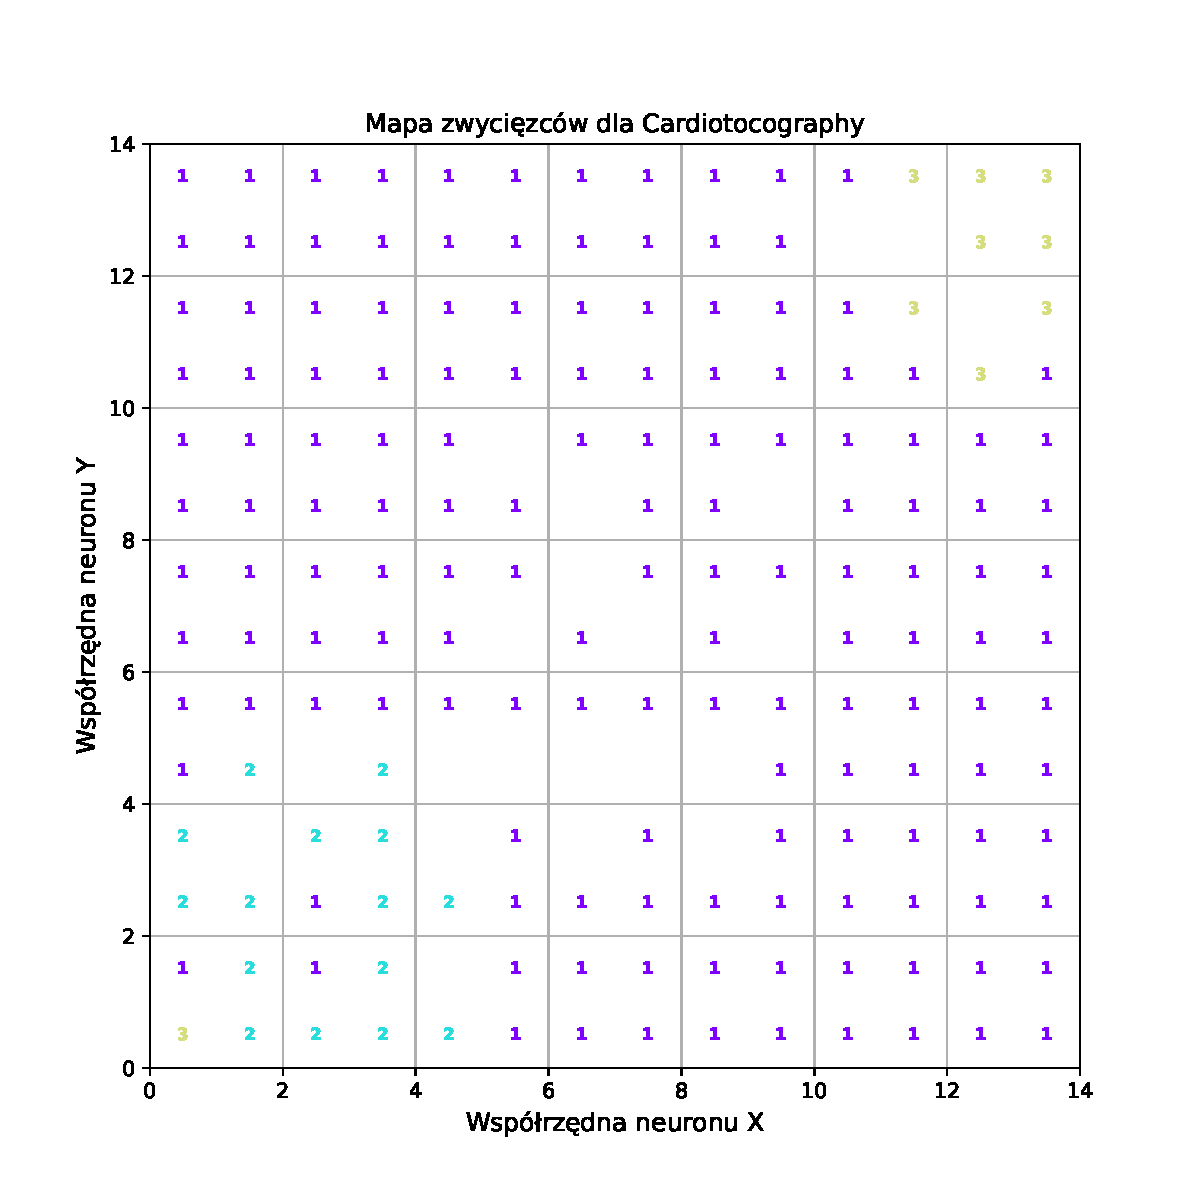
\includegraphics[width=0.8\textwidth]{./img/Fetal_best}
    \caption{Mapa zwycięzców otrzymana w wyniku testów na zbiorze Cardiotocography}
    \label{fig:Fetal_best}
\end{figure}
%MNIST wyniki
\section{Badania na zbiorze MNIST}\label{MNIST_sekcja}
Badaniami objęto również zbior MNIST (ang. "\textit{Modified National Institute of Standards and Technology dataset}", tłumaczenie: "zmodyfikowany zbiór danych Narodowego Instytutu Standardów i Technologii") \cite{MNIST}. Został on stworzony w 1998 roku, jako zmodyfikowana wersja zbioru NIST. Jest to jeden z najbardziej popularnych zbiorów danych przeznaczonych do klasyfikacji i klasteryzacji. Zbiór ten zawiera 70 000 obrazów ręcznie pisanych cyfr w skali szarości, o rozmiarze 28x28 pikseli. Każdy obraz przypisany jest do jednej z dziesięciu klas, odpowiadających cyfrom od 0 do 9. W tym zbiorze etykiety reprezentują wartości numeryczne przypisane do każdego obrazu, jednoznacznie identyfikując przedstawioną na nim cyfrę (od 0 do 9). W wyniku wykorzystania skali szarości,  po spłaszczeniu obrazu do jednowymiarowego wektora każda z danych ma 784 wymiary. 

Decyzja o przeprowadzeniu badań na tym zbiorze wynikała z konieczności zbadania możliwości stosowania sieci SOM w zbiorach danych z dużą liczbą wzorców wejściowych, w których każdy wektor wejściowy ma wiele cech. Rozłożenie liczebności w klasach jest równomierne, jednak istnieje możliwość błędnej klasyfikacji danych, ze względu na ich stopień podobieństwa. Przy tak wysokiej liczbie cech istnieje bardzo duże prawdopodobieństwo błędnej klasyfikacji.
Może to wynikać między innymi z różnic w stylach pisma i podobieństwa niektórych cyfr (np. "3"\ i "8"\ lub "4"\ i "9"). Badanie może również pokazać zdolności do zachowywania topologii wielowymiarowych danych wejściowych w tak dużym i zróżnicowanym zbiorze danych. W taki przypadku oczekuje się, że na mapie zwycięzców etykiety liczbowe danych podobnych do siebie wizualnie będą znajdowały się w niedalekiej odległości (na przykład klasa z etykietą "2"\ powinna być zlokalizowana w pobliżu klasy z etykietą "8").

Trening sieci przeprowadzono dla siatek 30 na 30 neuronów, z początkowym promieniem równym 15 i początkową wartością współczynnika uczenia równą 0.5. Wykorzystano funkcję dążącą do jedności dla zmiany wartości promienia \ref{eq:decay_to_one} oraz funkcję wymierną dla zmiany wartości współczynnika uczenia \ref{eq:exponential_decay}. Każda sieć była trenowana przez 200 epok. Z uwagi na wysoką liczbę neuronów w sieci przy procesie treningu skorzystano z zaimplementowanej możliwości obliczeń używających tensorów, wykorzystując przy tym procesor graficzny.

Wyniki otrzymanych błędów kwantyzacji i topograficznych przedstawiono w tabeli \ref{MNIST_wyniki}.


\begin{table}[h]
\centering
\caption{Wartości błędów topograficznych i kwantyzacji  z testów na zbiorze MNIST}
\label{MNIST_wyniki}
\begin{tabular}{|l|l|c|c|c|c|}
\hline
\textbf{\begin{tabular}[c]{@{}l@{}}funkcja\\ sasiedztwa\end{tabular}} & \textbf{Rodzaj błędu} & \multicolumn{1}{l|}{\(\textbf{hex}_{ncp}\)} & \multicolumn{1}{l|}{\(\textbf{rect}_{ncp}\)} & \multicolumn{1}{l|}{\(\textbf{hex}_{cp}\)} & \multicolumn{1}{l|}{\(\textbf{rect}_{cp}\)} \\ \hline
\multirow{2}{*}{\textbf{gaussa}}                                      & błąd kwantyzacji      & 4.890                                       & 4.953                                        & 4.906                                      & 5.022                                       \\ \cline{2-2}
                                                                      & błąd topograficzny    & 0.039                                       & 0.113                                        & 0.064                                      & 0.127                                       \\ \hline
\multirow{2}{*}{\textbf{trójkątna}}                                   & błąd kwantyzacji      & 4.913                                       & 4.954                                        & 4.913                                      & 5.236                                       \\ \cline{2-2}
                                                                      & błąd topograficzny    & 0.053                                       & 0.121                                        & 0.067                                      & 0.149                                      \\ \hline
\multirow{2}{*}{\textbf{prostokątna}}                                     & błąd kwantyzacji      & 5.110                                       & 5.221                                        & 4.923                                      & 5.334                                       \\ \cline{2-2}
                                                                      & błąd topograficzny    & 0.114                                       & 0.242                                       & 0.151                                      & 0.352                                       \\ \hline
\multirow{2}{*}{\textbf{eksponencjalna}}                              & błąd kwantyzacji      & 4.952                                       & 4.982                                        & 4.915                                      & 5.312                                       \\ \cline{2-2}
                                                                      & błąd topograficzny    & 0.073                                       & 0.125                                        & 0.062                                      & 0.144                                       \\ \hline
\end{tabular}
\end{table}
\subsection{Wnioski z badań na zbiorze MNIST}
Dla zbioru MNIST, z uwagi na dużą liczbę wymiarów wektorów wejściowych, maksymalny błąd kwantyzacji, wyznaczony za pomocą zależności \ref{maksymalny_blad_kwantyzacji}, przyjmuje wartość \(\sqrt{784} = 28\). 
Średni błąd kwantyzacji dla wszystkich badań wyniósł 5.033, co stanowi \(17.9\%\) wartości maksymalnej. Jest to wynik relatywnie wysoki, jednak spodziewany, ze względu na dużą ilość danych uczących, z wieloma wymiarami. Miara ta jednak nie skreśla zastosowania sieci SOM przy klasyfikowaniu takich obrazów, jak te w zbiorze MNIST.
Wartości błędów kwantyzacji nie różniły się znacząco miedzy sobą, niezależnie od zastosowanej funkcji sąsiedztwa, jednak błędy topograficzne miały zupełnie inne wartości, w zależności od zastosowanej funkcji sąsiedztwa.

Zastosowanie funkcja progowej doprowadziło do największych błędów topograficznych. Lepsze rezultaty osiągnięto przy niecałkowitej zmianie promienia sąsiedztwa, jednak nie są to na tyle niskie wartości, aby umożliwić poprawną klasyfikację obrazów przedstawiających liczby. Również mapy zwycięzców dla tej funkcji cechowały się niepoprawnym grupowaniem i zupełnym niezachowywaniem relacji w danych wejściowych.

Badania z wykorzystaniem funkcji trójkątnej i funkcji eksponencjalnej skutkowały bardzo zbliżonymi wartościami błędów, zarówno kwantyzacji jak i topograficznych. Z tych dwóch podejść jednak uzyskano nieznacznie lepsze rezultaty na mapie zwycięzców, wykorzystując funkcję trójkątną. Podobnie jak przy zastosowaniu funkcji progowej, w tych wypadkach również lepiej sprawdzały się topologie heksagonalne, wraz z niecałkowitą zmianą promienia. Mapy zwycięzców dla przypadków stosowania funkcji trójkątnej były w ogólności bardziej precyzyjne niż te stworzone za pomocą sieci trenowanych funkcją eksponencjalną. Mapy te były bardzo zbliżone do najlepszych wyników, uzyskanych za pomocą funkcji Gaussa.

Najniższe wartości błędów kwantyzacji i topograficznych uzyskano dla zastosowania funkcji Gaussa. Najlepsze grupowanie uzyskano, stosując w funkcje zmiany promienia przyjmującą wartości niecałkowite oraz topologie heksagonalną. Mapę zwycięzców dla tego przypadku przedstawiono na \ref{fig:MNIST_best}. W innych przypadkach osiągano zbliżone wartości błędów kwantyzacji, jednak błędy topograficzne istotnie się różniły. Osiągnięto lepsze rezultaty stosując topologię heksagonalną. 

Z badań przeprowadzonych na zbiorze MNIST można wyciągnąć pewne wnioski. Stosowanie niecałkowitych wartości promienia prowadzi do zmniejszenia wartości błędów topograficznych przy przypisywaniu danych z tego zbioru do klas. Jest to niezależne od zastosowanej funkcji sąsiedztwa. Dodatkowo, najlepsze rezultaty osiągnięto za pomocą funkcji Gaussa, co jest zgodne z trendami badań w literaturze \cite{Kolasa_artykul,DeepSOM}. Niewiele gorsze rezultaty uzyskano za pomocą funkcji trójkątnej i eksponencjalnej, przy czym pierwsza z nich dała nieznacznie lepsze rezultaty. Funkcja prostokątna nie umożliwiła poprawnego przypisania do klas danych ze zbioru MNIST.
\\ W przypadku rozważania wpływu topologii sieci na wartość błędów oraz na jakość mapy zwycięzców, można stwierdzić, że zastosowanie topologii heksagonalnej poprawiło efekty wszystkich miar. Może być to powiązane ze specyficzną strukturą danych ze zbioru MNIST.

Przedstawiona na rysunku \ref{fig:MNIST_best} mapa zwycięzców poprawnie odwzorowuje strukturę danych wejściowych, wykazując widoczne lokalne skupiska odpowiadające określonym klasom, takim jak 3, 7, 2 czy 0. Niemniej jednak, w niektórych obszarach pojawia się mieszanie klas lub brak jednoznacznego przypisania. Topologia danych została zachowana w znacznym stopniu, choć można również zauważyć błędy w przypisaniu. Rezultaty te oznaczają, że stosowanie jedynie sieci SOM, bez innych narzędzi analizy danych, nie gwarantuje idealnego przypisywania do klas tak złożone dane  jak obrazy rozmiaru 28x28. 
 
\begin{figure}[h]
    \centering
    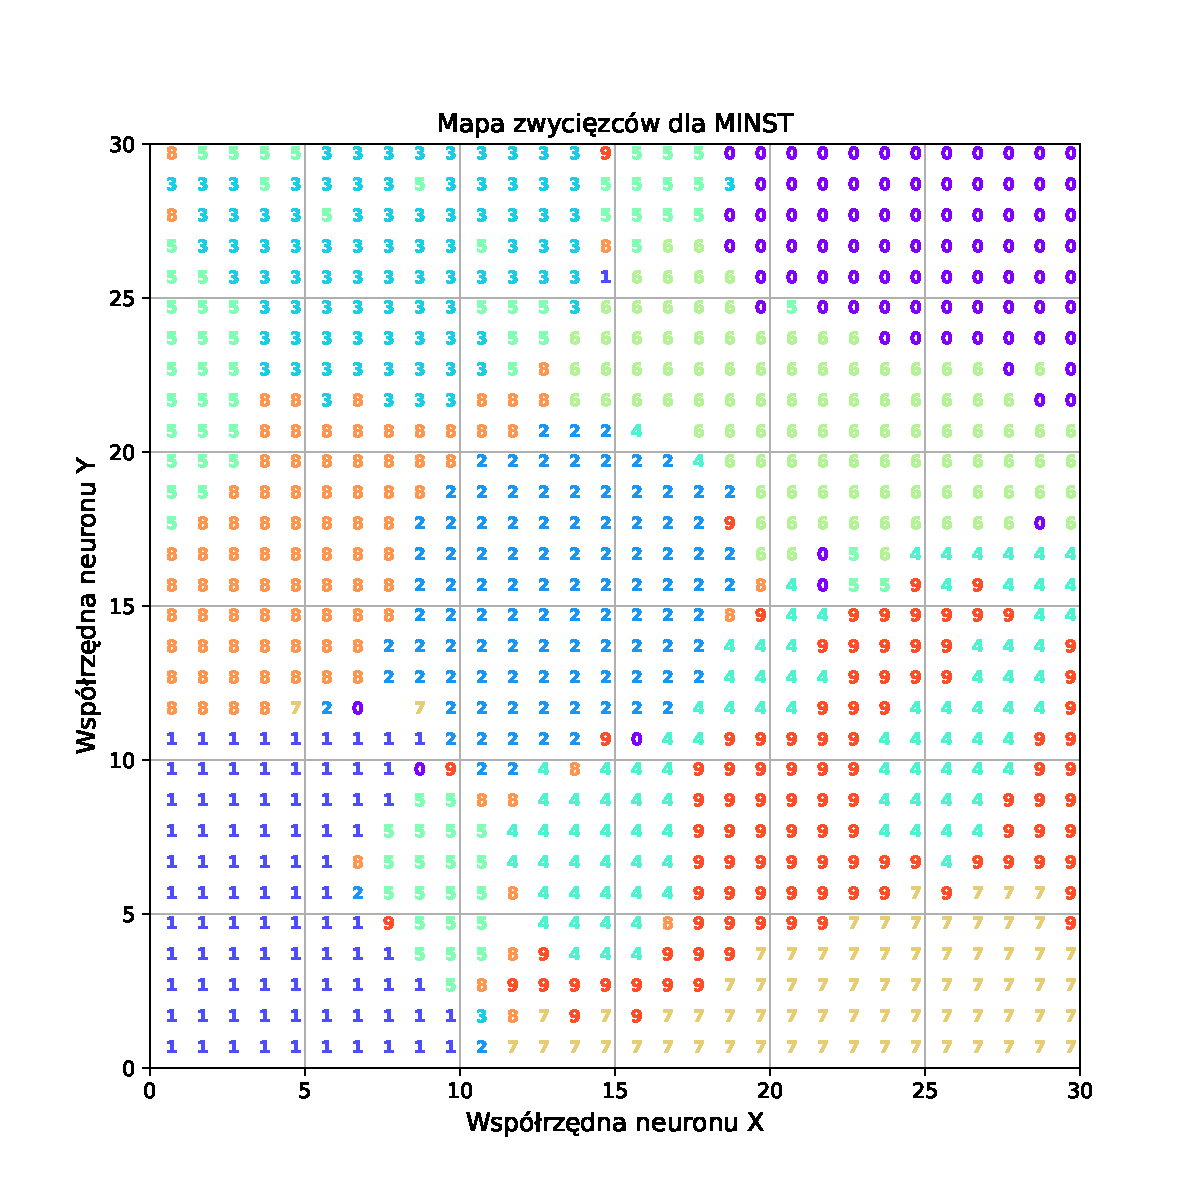
\includegraphics[width=0.8\textwidth]{./img/MNIST_best.pdf}
    \caption{Mapa zwycięzców otrzymana w wyniku testów na zbiorze MNIST}
    \label{fig:MNIST_best}
\end{figure}


\chapter{Analiza wyników przeprowadzonych badan}
\section{Analiza wpływu flag kompilatora na kod sekwencyjny}
\section{Analiza wpływu optymalizacji ręcznej programu sekwencyjnego}
\section{Analiza skalowalności rozwiązania wielowątkowego}
\section{Zestawienie zbiorcze i dyskusja wyników}
% tu będą kolejne rozdziały

\listoffigures
\addcontentsline{toc}{chapter}{Spis rysunków}
\listoftables
\addcontentsline{toc}{chapter}{Spis tabel}

\bibliographystyle{unsrt} % Wybór stylu bibliografii
\bibliography{bibliografia}

%*****************
% wymagane dodatki:
% Opis dyplomu
% Zawartość płyty CD
% Instrukcja dla projektanta
% Instrukcja dla użytkownika
\begin{appendices}
\chapter[Instrukcja dla użytkownika]{Instrukcja dla u\.Zytkownika}

Programy w języku Python, zawierające implementację klas do obsługi logiki oraz wizualizacji wyników znajdują się w archiwum ZIP, dołączonym do niniejszej pracy.
W celu poprawnego działania należy pobrać ten folder i go rozpakować. Aby powtórzyć badania opisane w pracy należy następnie podjąć następujące kroki:
\begin{enumerate}
    \item Pobrać wybrany zbiór uczący
    \item Znormalizować dane ze zbioru
    \item Podzielić zbiór na dane uczące i testowe
    \item Stworzyć obiekt klasy SelfOrganizingMap z poprawnym doborem parametrów 
    \item Przeprowadzić trening, wykorzystując metodę train
    \item Przeprowadzić ewaluacje modelu 
\end{enumerate}
Do pobrania zbiorów uczących można użyć pomocniczych pakietów, takich jak \texttt{scipy}, choć nie jest to konieczne. Można też skorzystać z źródeł internetowych, z których można bezpośrednio pobrać pliki z danymi. W badaniach normalizację przeprowadzono za pomocą zależności podanej w rozdziale \ref{WykonaneBadania}, jednak można również skorzystać metody MinMaxScaller z \texttt{scipy}. Przykładowe tworzenie obiektu klasy przedstawiono na \ref{lst:som_initialization}. Pod zmienne należy podstawić wybrane parametry sieci SOM.
\begin{lstlisting}[language=Python, caption={Przykład inicjalizacji klasy \texttt{SelfOrganizingMap}}, label={lst:som_initialization}]
som = SelfOrganizingMap(
    dim_x=DIM_X, dim_y=DIM_Y, num_of_iterations=NUM_OF_EPOCHS, input_dimension=DIM,
    distance_metric=WYBRANA_METRYKA, initial_radius=INITIAL_R, 
    initial_learning_rate=LEARNING_RATE,
    network_topology= WYBRANA_TOPOLOGIA,
    neighbourhood_function=SASIEDZTWO,
    int_radius=RADIUS_FLAG
)
\end{lstlisting}
W celu uruchomienia programu niezbędne jest posiadanie pakietów, wraz z odpowiednią wersją Pythona. Wszystkie wymagane biblioteki, wraz z użytą wersją Pythona, dostępne są w pliku \texttt{requirements.txt}. Zaleca się tworzenie wirtualnego środowiska za pomocą narzędzia \texttt{venv} oraz instalowanie pakietów z pomocą menadżera \texttt{pip}. W celu instalacji poprawnej wersji pakietu Pytorch należy skorzystać ze strony internetowej  \href{https://pytorch.org/get-started/locally/}{pakietu Pytorch}. Spowodowane jest to koniecznym wyborem wersji pakietu, zależnej od dostępnych środowisk pracy, takich jak wersja Pythona czy obsługiwane sterowniki GPU.
Ewaluacji modelu można dokonywać za pomocą analizy błędu kwantyzacji i błędu topograficznego, korzystając z metod \texttt{quantization\_error} oraz \texttt{topographic\_error}. Dodatkowo, możliwe jest wyświetlenie mapy zwycięzców za pomocą metody \texttt{make\_winmap} z klasy \texttt{VisualizeSOMResults}.

%\include{AppB}
\end{appendices}
%*****************

\end{document}
